\documentclass[journal,transmag]{IEEEtran}
\usepackage{flushend}

\usepackage{graphics}
\usepackage{graphicx}
\usepackage{epstopdf}
\usepackage{epsfig}

\usepackage[table]{xcolor}
\usepackage{ifpdf}
\usepackage{color}
\usepackage{multirow}
\usepackage{cite}

%\usepackage[latin9]{inputenc}
\usepackage{amsmath}
\usepackage{amssymb}
\usepackage[11pt]{moresize}
\usepackage{standalone}
\usepackage{dsfont}
\usepackage{mathrsfs}

\usepackage[tight,footnotesize]{subfigure}

\usepackage[linesnumbered,ruled,vlined]{algorithm2e}

\usepackage{algorithmic}




\definecolor{xy}{cmyk}{0,0.42,1,0}






\begin{document}

\title{A QoS Association scheme based on Clients behaviours and priority for proportional Fairness of Radio Resources in WLAN networks}

\author{\IEEEauthorblockN{Mohamed Amine Kafi\IEEEauthorrefmark{1},
Alexandre Mouradian\IEEEauthorrefmark{1},
V\'eronique V\`eque\IEEEauthorrefmark{1}}
\IEEEauthorblockA{\IEEEauthorrefmark{1}L2S, CentraleSUPELEC, Paris sud University, FRANCE.}

\thanks{%Manuscript received December 1, 2012; revised September 17, 2014. 
Corresponding author: Mohamed Amine Kafi (email:kafiamine@gmail.com)}}



\IEEEtitleabstractindextext{%
\begin{abstract}
With the increasing number of WLAN devices and the application hungry resources demand, the WLAN networks became denser and denser in order to form a multi cell network that answers these demands. Indeed, the clients should associate to one between the different available Access Points (APs), and the IEEE standard association is with the stronger signal based AP which shows limited network performance. 
The aim of this paper is to propose jointly an association and ressources sharing scheme between clients of such multi cell and multi rate WLAN at the SDN central controller level to balance the network charge. We interest in the case that the clients have different priorities and bandwidth demands. The goal of our scheme is also to ensure as possible a proportional fair based scheduling while giving advantage for prioritized clients. We have proposed an off-line and an on-line schemes centrally at the SDN controller level to be used independently in a periodic manner, and at each arriving or departure of clients, respectively. The simulation results compared to the IEEE standard and two periodic and online state of the art works shown performance enhancements and clients satisfaction specially for the more priority ones.

\end{abstract}

% Note that keywords are not normally used for peerreview papers.
\begin{IEEEkeywords}
Wireless Local Network (WLAN), Throughput, Controller, 802.11, SDN, QoS, client priority, access point. 
\end{IEEEkeywords}}

% make the title area
\maketitle

\IEEEdisplaynontitleabstractindextext
% \IEEEdisplaynontitleabstractindextext has no effect when using
% compsoc or transmag under a non-conference mode.

\IEEEpeerreviewmaketitle

\section{Introduction}

The number of smart devices, applications and data traffic have known an important multiplication in the last years and will continue in the next ones. The use of 3G, 4G, and will continue with 5G, has reinforced and promoted this large use of smart devices like smart phones, terminal games, laptops and any IoT based terminal. On the other hand, the cellular WLAN use has known the same explosion rather than decreasing \cite{17why_Long_WIFI_Connect,14group_based_RRM}, specially with the 5G technology which uses the WLAN as a backbone \cite{16AP_association_optimisation_fairness}. In fact, the availability of WLAN Access Points every where (habitation buildings, commercial and industrial environments...) at the same time of their cheap cost helped a lot to WLANs success \cite{15Node_throughput_enhencement_wifi}. In parallel, this large use of WLAN technology requires the densification of the cells in order to answer this increase in bandwidth demands of hungry devices and applications.     

The architectures used for WIFI network in real scenarios could be as simple as a single Access Point, like that used for apartments or small offices and serves the multitude of devices in its vicinity, to a complex multi cell architecture in which many Access Points are installed and cover all the environment as a multi cell network. An example of this second architecture could be seen in airports, train stations, malls and commercial centers, large companies... In this case, the Access Points could be organised in a same network or cohabit in different networks. Each Access Point is responsible of the clients associated with it. On the other hand, each client could see different Access Points in its coverage area and should be associated to one before beginning the use of the bandwidth. The cells diameter change according to the clients densification and overlapping of Access Points coverage which is mandatory to avoid clients disconnection in roaming case \cite{15fuzzy_load_balancing_802.11}. The association choice is very important because it decides how the bandwidth resources are divided between all the clients of the whole network and the load balancing that results between all the Access Points of the same network \cite{14AP_association_multirate_WLAN}. Clients traffic exchange with the Access Points could be in the uplink or downlink direction, with the downlink traffic domination in several Internet based applications, like video streaming, web mail and web browsing \cite{05DIRAC}.   

The densification of Access Points in order to growth the network size and accept more clients is at the same time a strong point of the cellular WLAN robustness, but can be a cause of weakness \cite{15Node_throughput_enhencement_wifi}. So, this densification should be monitored and the Access Points load charge balanced to ensure the well performance of the clients. In fact, adjacent Access Points may use the same channels because of the lack of orthogonal channels, which leads to high interference levels and consequently throughput degradation \cite{15Node_throughput_enhencement_wifi,16AP_association_optimisation_fairness}. On the other hand, the standard clients association using IEEE 802.11 connects every node to the strongest signal based Access Point leading to overloading of this last one in case the clients distribution is not uniform and concentrated in one Access Point vicinity, while the other surrounding less signal Access Points may be empty with wasted bandwidth capacity \cite{14optimalAP_INFOCOM,14AP_association_multirate_WLAN,16throughput_optimisation_association_bandwidth}. This could be explained by the fact that the bandwidth capacity of the overloaded Access Point, which is a limited resource in time, is divided by all the associated clients, and the other Access Points resources are not used \cite{04Intelligent_resource_management,16AP_association_optimisation_fairness}. 
 
In addition, the DCF (Distributed Coordination Function) used for resource management at the Access Point level leads that slow bandwidth clients make the other clients send their traffic at their slow rate \cite{15time_fairness_MAC,16AP_association_optimisation_fairness}. These behaviours leads to aggregated and individual performance degradation \cite{15Node_throughput_enhencement_wifi,15OpenSDWN_home_entreprise_WIFI,14online_AP_association_80211n,10Assesment_EDCA_real_time,16Indoor_spatial_reuse_adaptive_antenna}.    
On another side, the clients capacity demands depend deeply on the used applications, and could be therefore dynamic during the client connexion lifetime. Taking this parameter into account during the clients association optimisation operation seems being mandatory, rather than the supposition that all the clients have equal traffic demands. This point is little invoked in literature works \cite{17QOS_AP_selection}. 
Also, the clients priorities parameter is also an important point that is little invoked in literature works. So sharing the resources and making associations while taking these priorities into account could enhance the individual throughput of the most important clients \cite{16VALI_SDN}.

In order to handle efficiently the radio bandwidth resource and share it adequately between all the Access Points and therefore the clients, intelligent centralised RRM (Radio Ressource Management) is required to have high network aggregated and individual performance. This control should cover the channel assignment between the neighboring Access Points to avoid interferences, the clients associations with the appropriate Access Point to load balance the Access Points charge, and finally the resources management between the clients of the same Access Point through communication scheduling and bandwidth sharing. Allowing clients transparent roaming between the Access Points is also required to avoid disconnections, whatever the cause of the roaming (mobility or QoS) \cite{14optimalAP_INFOCOM,14Odin:Programmatic_Orchestration_WiFi}. Performing the previous tasks decisions centrally at the level of the SDN (Software Defined Networking) controller allows more programmability, flexibility and changing network strategies as services while necessary network configurations are required, without hardware change or configuration \cite{14Odin:Programmatic_Orchestration_WiFi}. 

Figure\ref{SDN_based_multi_cell_WLAN} depicts a possible architecture of a such network with the controller. In this paper, we focus our selves on the problem of clients associations while clients bandwidth demands and priorities are taken into account. Indeed, we propose two central schemes at the SDN WLAN controller. One scheme to be used periodically in an offline manner to allow maximal association optimisation, while the other scheme is to be used in an online manner, at each client arrival. The two schemes could be used independently or jointly as a complete control. The SDN controller on its side, performs also the other tasks, like channel assignments, scheduling decisions, and roaming orders.     
The remaining of the paper will be organised as follows. The related work is discussed in section \ref{Related_Work}, where we describe and classify some literature works. In section \ref{Proposed scheme model}, we present the system model of the two schemes and highlight the proposed algorithms. We evaluate the performance of the schemes in different scenarios in section \ref{performance evaluation}. In section \ref{Conclusion}, we summarise the paper ideas by giving also some perspectives. 

%==============================================
\begin{figure}[t]
\centering 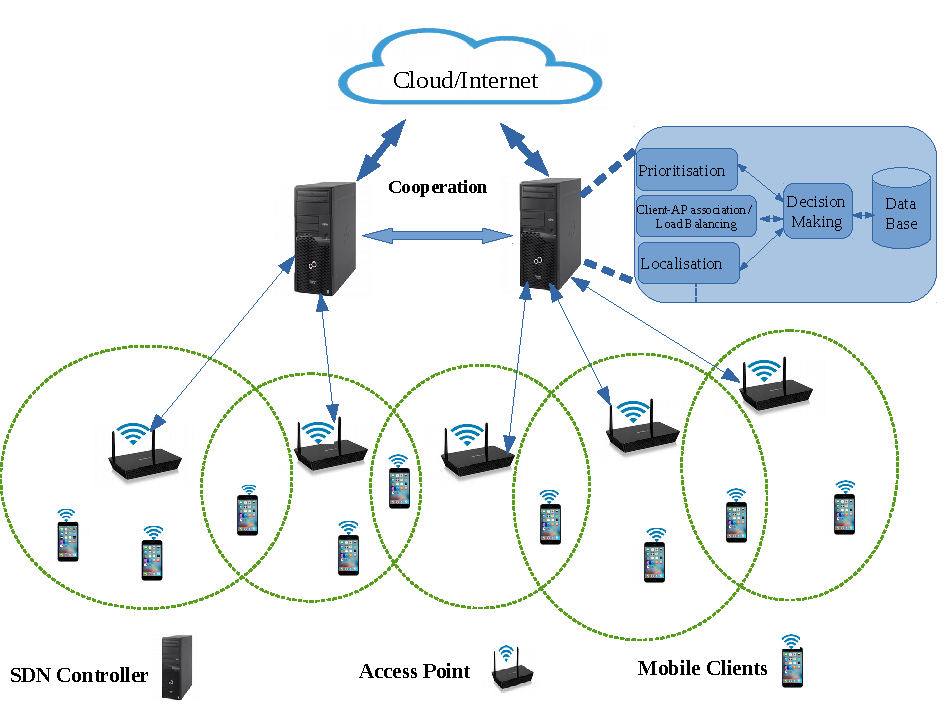
\includegraphics[width=9cm]{Figures/SDN_controller} \caption{WLAN Network scheme using SDN controllers}
\label{SDN_based_multi_cell_WLAN} 
\end{figure}

%==============================================

\section{Related Work}
\label{Related_Work}

The state of the art works for the Radio ressource management proposed for cellular WLAN area networks could be classified to three main classes. The first class interests to the wireless channel management between the Access Points that form the different cells. The aim of this class is to optimise the channel distribution and reuse according to the interference levels and the number of available channels. The second class of works interests on the optimisation of clients association with these Access Points in order to enhance the clients satisfaction in terms of individual throughput and delay. The third class interests on resource sharing at the level of each Access Point through schedule management of clients communications. In addition, many works interest on the combination of these classes in order to enhance more the network performance, like the combination of channel management according to clients distribution and associations, or also the combination of clients association and ressource scheduling. On the other hand, the decision of each class works could be performed centrally or in a distributed manner. The central decision could be made at the level of a delegated Access Point or at a controller, specially with the large use of SDN paradigm, that allows easy reconfiguration of the network management tasks. As our proposed scheme is situated in the second class that handles clients associations, we describe in the following many works of this subclass.        
As said previously, the client association decision could be made centrally at the controller like in \cite{14AP_association_multirate_WLAN,16throughput_optimisation_association_bandwidth,16AP_association_optimisation_fairness,17QOS_AP_selection} or in a distributed manner at the client level like in \cite{17decentralised_AP_selection}. In addition to the level of the decision, the periodicity of the association decision can be classified to online schemes like in \cite{17QOS_AP_selection} where the clients arrive or depart at any moment of the application lifetime. The decision could be also performed in a periodic offline manner in which the clients are supposed present at the moment of the decision like in \cite{14AP_association_multirate_WLAN,16throughput_optimisation_association_bandwidth,16AP_association_optimisation_fairness}. 
The association decision could have as a goal to ensure fairness between the clients like in \cite{14AP_association_multirate_WLAN,16throughput_optimisation_association_bandwidth,16AP_association_optimisation_fairness}. Other works interest on the optimisation of the QoS without ensuring necessary any fairness form between the clients \cite{17QOS_AP_selection}. The clients traffic could also be supposed consuming all the given capacity of the sharing resource scheme, named also saturated traffic, like in \cite{14AP_association_multirate_WLAN,16AP_association_optimisation_fairness}. Other works take from the beginning of the scheme the capacity demands of the clients in order to optimise the associations, like in \cite{16throughput_optimisation_association_bandwidth,17QOS_AP_selection}.    

The authors of \cite{14AP_association_multirate_WLAN} propose an offline scheme to be applied centrally at the controller in order to ensure throughput optimisation between clients based on proportional fairness. The authors formulate the problem as a non linear optimization program for which a heuristic algorithm, dubbed NLAO-PF is proposed. But this solution requires modification on the clients software which is not so practical in real scenarios. 

The scheme proposed in \cite{16throughput_optimisation_association_bandwidth} takes into account the clients capacity demands and proceed in a centralised offline manner. The authors formulate the problem as a non linear mixed integer optimization problem, where the demands are added as constraints in the problem. The authors proposed an algorithm dubbed MABU (Maximum Aggregated Bandwidth Utility) that fulfills the association and capacity sharing in two steps. The first step consists to assign the clients to the adequate Access Points, while the second step consists to share each Access Point capacity between the clients according to time fairness and capacity demands. The fact of taking only the offline association decreases the practical algorithm efficiency. Also, the capacity demands could not be changed after the ressource sharing, unless the algorithm should be re-executed, and the clients may be de-associated. 


The authors in \cite{16AP_association_optimisation_fairness} leave the standard access fairness capacity sharing which is use by default in the DCF (Distributed Coordination Function) of the IEEE.8011 standard. The problem is formulated as a non linear optimisation program in two versions. The first one takes interference between the Access Points into account and the second does not. The authors propose an heuristic algorithm based on local search method in order to solve the problem. In this method, at each iteration, one client could change its association in order to enhance the objective function, until the end condition of the method which could simply be based on a number of iterations or on time execution. The advantage of this method is to have always one useful solution. But the algorithm in its current version does not take clients demands nor allow changing two clients associations (or more) at the same iterations, which could give good results as this case could be inaccessible with one change at time.      


In \cite{17QOS_AP_selection} a SDN based centralised association is proposed as a part of the WI-5 project. The authors take clients capacity demands into account and perform the online association at each arriving client. In this project, the authors also propose a channel optimisation scheme to be used with the association optimisation part in a whole framework. The authors association scheme uses a parameter named "Fittingness Factor"(FF), in which the chosen Access Point is that having the closer link capacity with the client demand and that reducing the least the other clients throughput (named network fittingness). But network efficiency is not taken into account in this scheme, which could lead to suboptimal solutions. The fact of not re-associating already associated clients could decrease also the global performance.     

In \cite{19reinforcement_learning} we proposed a centralised online scheme that learns from real environment capacities using Q-learning method in order to choose the optimal Access Point for the clients, while taking their capacity demands into account. The scheme chooses at each moment to re-associate the least satisfied client in case of non arriving of new clients. Also, the resources of leaving clients are redistributed between the other ones.    

In the following section, we propose an on line and offline schemes to be used separately or together centrally at the SDN controller. The scheme takes into account the clients bandwidth demands in addition to their priorities for the resource sharing. Even our scheme focuses on the association part, but the scheduling part should be performed at the Access Points level, in addition to the channel optimisation decisions performed at the SDN controller level. 

\section{system Model from}
\label{Proposed scheme model}
In this section, we highlight the network model used in our schemes description for clients Association optimisation and resource sharing at the level of the central SDN controller.

At the beginning, we suppose that the SDN controller has executed the channel assignment optimisation scheme in order to reduce as possible the interferences between neighboring Access Points through channel reuse. For that, we suppose in this version that the interference is neglected and that the Access Points have sufficient orthogonal channels. We can enhance the scheme in future by supposing that many of the neighboring Access Points should use the same orthogonal channel, resulting to the inter Access Points interference in addition to the intra interference that is taken into account by our current scheme through time division communications. We suppose having in our system $M$ AP under the SDN controller responsibility. The number of clients supposed in the system is $N$. In the offline scheme, this number of clients is present since the beginning of the application and keeps until the end. While in the online scheme, we suppose having a variable number of users according to the arrivals and departures, but an average number of $N$ users is maintained. Each client $i\in\{1,...,N\}$ could be associated to one of the Access Points $j\in\{1,...,M\}$ at a time. For that, we denote the variable $x_{ij}$ to be equal to 1 if the client $i$ is connected to the Access Point $j$, or equal to 0 contrary. Each variable $x_{ij}$ is an element of the association matrix $X$. As the users could be in different locations away from the Access Points and encountering many obstacles, the link capacities could be different because of the MCS(modulation coding scheme) used. For that, we suppose that each client $i$ has a link capacity $c_{ij}$ with AP $j$. According to the IEEE802.11n, the $c_{ij}$ rate value could be taken from the set $\mathscr{LC}=\{6.5, 13, 19.5, 26, 39, 52, 58.5, 78, 104, 117, 130\}$ (here in Mbps). Let also suppose that each client of our system is at least covered by one Access Point $j$ with which its capacity $c_{ij}$ is different to 0, and so: $\sum_{j=1}^{M}c_{ij}>0$. We have therefore the matrix $C$ that contains all possible values of $c_{ij}$. As the dominating traffic in most of the WLAN applications is in the downlink direction (like that of video streaming, web browsing and mail...), we interest on this type of traffic. 

In real scenarios and according to the used application, each user $i$ could have a given capacity demand in order to have an acceptable QoS, let this demand be $d_{i}$. We suppose that our system is equipped with a mechanism that translates reliably each client used application demand to a well known bandwidth demand, like that supposed in \cite{17QOS_AP_selection,16centralised_wifi_manegement}. Such mechanism could be integrated proactively at the SDN controller, or dynamically through machine learning like methods. We recall here that this demand is independent from the Access Point with which the client is associated but fixed only to the application used. We suppose in our offline and online schemes that the demands are fix. But in future versions, we can enhance the system by accepting the change in demands, specially for the online scheme that is supposed reacting to the network parameters dynamicity.

Each client in our system has also a given priority $w_{i}$, which also has no relation with the Access Point but rather a relation to the client type. In this version, the priority of the client is independent to the application, too. But, in future versions, we can introduce the priority in relation to the used application. A real example on this is that a user in a staff company has a high priority when using his professional mail application, and has a less priority when using the video streaming application. 

The aim of our offline and online schemes is to perform optimised clients associations with adequate Access Points in order to maximise the downlink aggregated system throughput while promoting higher priority clients and ensuring fairness as possible between the same priority class clients, while taking their bandwidth demands into account.

For sharing the time ressources of each Access Point between its associated clients, the time resource of the Access Point is divided between the clients so that each client has a time period connection $t_{ij}$ between 0 and $T_{ij}$, where $T_{ij}=d_i/c_{ij}$ is the time demand with the corresponding Access Point $j$ and $\sum_{i=1}^{N}t_{ij}\leq1$. So the bandwidth resulted for each client $i$ on Access Point $j$ is $b_{ij}=t_{ij} * c_{ij}$. 
In our schemes, the more priority clients are given their bandwidth demands before of the less priority ones, these last could see their bandwidth put to zero in case that all the time period of the Access Point is consumed. This is because of supposing that the high priority clients applications are critical needing so total satisfaction as possible. In future versions, we can suppose weighting priorities bandwidths in order to have the time sharing of the form $t_{ij}=w_i/w_k * t_{kj}$, where $w_i$ and $w_k$ are the priorities of the clients $i$ and $k$ respectively. 
For each priority class, at the concerned Access Point level, max-min time fairness distribution is used for channel sharing in order to avoid the problem of access fairness in multi rate capacity network, known in literature as DCF anomaly of 802.11 \cite{03performance_anomaly_DCF}. In fact, time fairness is used between the clients having the same priority, while taking their time demand into account so that each client could have as time period $t_{ij}$ a value in the interval $[min(T_{ij},T_{AP}/Nb\_clients),T_{ij}] $, where $T_{AP}$ is the current time period of the Access Point and $Nb\_clients$ is the number of clients of the current priority class associated to the Access Point. Each client uses its given time period, as explained previously, using its capacity link. 

In order to ensure the max-min time fairness, the time demands of a given priority class are sorted in the ascending order. The algorithm executes iteratively, where at each iteration of the algorithm, the remaining time of the Access Point is divided by the remaining number of clients of the current priority. If the resulted value is higher than the current client time demand, the client is given its time demand which is also subtracted from the total Access Point time value, and the number of clients of the current priority class is decreased by one. The algorithm stops when the number of clients to serve is null, or the time division could not satisfy the current client. In this second case, the remaining clients of the current class must share the same remaining time equally. This time sharing method (max-min time fairness without priority classes) is invoked in many previous works like in \cite{16throughput_optimisation_association_bandwidth,04time_based_fairness_multirate_WLAN,14AP_association_multirate_WLAN}, and could be implemented at the Access Point level like in \cite{11efficient_airtime_scheduling}.    
We define the user deficit as the difference between its bandwidth demand and its given bandwidth by the chosen Access Point $j$ as $z_i=b_{ij}-d_i$, and each user is satisfied if its deficit is null. The goal of our schemes is to reduce as possible the deficits according to the clients priorities levels.

For the users of less priority classes that see them selves having a null bandwidth, because of a null value of sending time at the level of the Access Point, we have chosen that they stay in a queue at the level of their Access Point for the offline scheme and at the level of the SDN controller in a unique queue for all the Access Points for the online scheme. In fact, these queues represent the price of satisfying the higher priority classes at first. Also, we suppose that at a given time, the other satisfied clients have finished their bandwidth use making therefore place for the waiting clients. In real scenarios, we can implement a scheme like that in \cite{06practical_queue_based_AP_association}, that uses the Reason field in IEEE 802.11 disassociation message to indicate the waiting time for the client.   

The table \ref{problem_notations} summarizes our previous notations. 

%=================================================
\begin{center} 
%\begin{footnotesize}
\begin{table}[htbp]
\centering
\begin{tabular}{|c|l|} %\
\hline
Notation 		& Description \\
\hline
$A$				& Set of available access points\\
$M$				& Number of concerned Access points, $|A|=M$ \\
$U$				& Set of all wireless clients \\
$N$				& Number of Concerned wireless clients, $|U|=N$  \\
$d_i$			& bandwidth demand of user $i$ \\	
$c_{ij}$ 		& Link capacity of client $i$ on AP $j$ \\
$C$		 		& matrix of Link capacities of clients with the APs\\
$T_{ij}$ 		& time demand of client $i$ on AP $j$,$T_{ij}=\frac{d_i}{c_{ij}}$ \\
$t_{ij}$		& Air-time for user $i$ on AP $j$  , \\
$w_i$			& priority of user $i$ \\
$b_{ij}$		& Bandwidth of user $i$ on AP $j$ \\			
$x_{ij}$		& binary variable that associates client $i$ to AP $j$ \\
$X$				& matrix of binary variables of clients associations\\
$z_i$			& bandwidth deficit value of the cuser $i$ \\ 

\hline
\end{tabular}
\caption{\label{problem_notations} Notations used to formulate the AP association optimisation problem}
\end{table}
%\end{footnotesize}
\end{center}
%======================================

\subsection{offline clients Association scheme with clients demands and priorities}
As explained previously, in this version, we suppose that all the clients are present in the system at the execution scheme time. In fact, this hypothesis is logical in the case that the system should be reset because of an electrical or software failure or update. In a general scheme containing the online and offline schemes, the execution of the offline part could also be triggered when the online part could not more answer the clients and system requirements. Also, as presented previously, we interest our selves with the downlink traffic direction, and that each client is covered by at least one Access Point, and that the clients should be associated with only one Access Point.      
We suppose that each client is interested on a data size that is translated to its capacity link demand $d_i$. We  are inspired in this offline part by the algorithm proposed in \cite{16throughput_optimisation_association_bandwidth}, and we enhance it by introducing the priority classes, which change the clients support order and the attributed bandwidths. The algorithm is divided into two main steps. The first one consists to associate the clients to the adequate Access Points, which is performed by CAPAB (Client Association with Priority and Aggregated Bandwidth) in the algorithm \ref{Algorithm_MABU_prio}. While the second step consists to share the capacity ressources according to the clients priorities and time demand in the level of each Access Point and is performed by PF2D2BA (Priority First, Fairness and Data Demand based Bandwidth Allocation) in the algorithm \ref{Algorithm_FBA_prio}.      

\subsubsection{CAPAB algorithm description}
The aim of this part of the offline scheme is distribute the clients towards the Access Points in order to load balance their charge. This is even the sum of time demands of the clients associated to the given Access Points exceeds one, signifying that the Access Point could not really satisfy the total demands. For that, the clients bandwidth demands are sorted according to their descending order but starting by the high priority classes ones. The iteration algorithm starts by the high priority clients and for each class, the bandwidth is sorted from the higher one. Each time a client chosen to be associated, the CAPAB algorithm chooses the Access Point least loaded after the association. The variable $x_{ij}$ of the client $i$ will be equal to 1 with the chosen Access Point $j$ and zero for the other Access Points. We recall here that the corresponding time demand for a given bandwidth demand, differs according to link capacities between the client and the Access Points, and is presented by $T_{ij}$ for the client $i$ with the Access Point $j$. The algorithm \ref{Algorithm_MABU_prio} highlights the CAPAB behaviour.
\documentclass[a4paper]{article}

%\usepackage[]{algorithm2e}
\usepackage[ruled,vlined]{algorithm2e}
%\usepackage{times}
%\usepackage{fancyhdr,graphicx,amsmath,amssymb}
\usepackage[utf8]{inputenc}
\usepackage[english]{babel}
%\usepackage[noend]{algpseudocode}

\begin{document}


\begin{algorithm}%[H]
\begin{scriptsize}
\caption{{\bf {\scriptsize CAPAB (Client Association with Priority and Aggregated Bandwidth)}} \label{Algorithm_MABU_prio}}
 \KwIn{$ \{T_{11},T_{12},... T_{NM}\}, \{w_1,w_2,...w_N\}, \{d_1,d_2,...d_N\} $} 
 \KwOut{\{$ x_{11},x_{12},... x_{NM}$\}}
% \KwData{this text}
% \KwResult{how to write algorithm with \LaTeX2e }
 -{\bf Initialisation:} $x_{ij}=0, \forall i \in \{1,...N \}, \forall j \in \{ 1,...M \} $\;
 -Sort the clients according to priority levels from the highest, for each level in descending order of bandwidth demand\;
 - \For {each sorted user $i$}{
      $j_{min}=argmin_j(\sum_{k=1}^{i-1}x_{kj}. T_{kj}+T_{ij})$\;
      $x_{ij_{min}}=1$ \;
    }
    \For {each $AP_j$}{
		use Algorithm PF2D2BA to schedule clients transmission time\;
	} 
\end{scriptsize}    
\end{algorithm}


\end{document}

    
\subsubsection{PF2D2BA algorithm description}
This part of the offline scheme has to ensure max-min time sharing fairness at the level of each Access Point, by starting from the high priority classes. Each time the current class demands are treated and the time resource is still available at the Access Point level, the next priority class is treated. If the time resource of the Access Point is not yet available, the next priority classes clients are given a null time resource, and are obliged to wait in a waiting queue at the level of the Access Point, until the other clients finished their use of the bandwidth, or centrally at the SDN controller in a common queue (as performed in the current implementation). The summary of the max-min fairness sharing is explained in the previous section, and the algorithm \ref{Algorithm_FBA_prio} describes PF2D2BA (Priority First, Fairness and Data Demand based Bandwidth Allocation) functioning. The effective bandwidth of each client $i$ with its Access Point $j$ will be simply the multiplication of its given time period $t_{ij}$ by its $c_{ij}$.      
 
\documentclass[a4paper]{article}

%\usepackage[]{algorithm2e}
\usepackage[ruled,vlined]{algorithm2e}
%\usepackage{times}
%\usepackage{fancyhdr,graphicx,amsmath,amssymb}
\usepackage[utf8]{inputenc}
\usepackage[english]{babel}
%\usepackage[noend]{algpseudocode}

\begin{document}

%and a simple example, taken from the v4.01 manual, is

\begin{algorithm}%[H]

\caption{{\bf {\scriptsize PF2D2BA (Priority First, Fairness and Data Demand based Bandwidth Allocation)}} \label{Algorithm_FBA_prio}}
\begin{scriptsize}
 \KwIn{T, \{$\tilde{T_1},\tilde{T_2},... \tilde{T_m}$\}, \{$w_1,w_2,...w_m$\}}
 \KwOut{\{$ \tilde{t_1},\tilde{t_2},... \tilde{t_m}$\}}
% \KwData{this text}
% \KwResult{how to write algorithm with \LaTeX2e }
 -sort $\tilde{T_i}$ according to priority levels from the highest, for each level in ascending order\;
 -{\bf Initialisation:} $T_{Total}=T$, $B_{prio}$= Set indexes CurrentPrio, \\ B= Set indexes AllClients - $B_{prio}$, $A=\emptyset $ , $k_{Total}=k_{prio}=1$, CountPrio=nbClients($B_{prio}$), $m_{prio}$=index last client (currentPrio)\;
 - $t_{B_{prio}}=T_{Total}/CountPrio$\; 
 - \While{$k_{Total} \leq m $ }{
     \While{$k_{prio} \leq m_{prio} $ }{
       \eIf{$\tilde{T}_{k_{prio}} > t_{B_{prio}} $}{
           Break\;
       }{
          $A= A+\{k_{prio}\}, B_{prio}= B_{prio}-\{k_{prio}\} , \tilde{t}_{k_{prio}}=\tilde{T}_{k_{prio}}, T_{Total}=T_{Total}- \tilde{T}_{k_{prio}}$, CountPrio=CountPrio-1, $k_{prio}=k_{prio}+1, k_{Total}=k_{Total} +1$, \ 
          $t_{B_{prio}}=T_{Total}/CountPrio $ \;
       }
     } 
     
     \eIf{$k_{prio} > m_{prio} $}{
         CurrentPrio=NextPrio, $B_{prio}$= Set indexes CurrentPrio, B= B- $B_{prio}$ , $m_{prio}$ =index last client (currentPrio), CountPrio=nbClients($B_{prio}$) \;
     }{
        \For {i $\in B_{prio}$}{
           $\tilde{t}_{i}=t_{B_{prio}}, T_{Total}=T_{Total}-t_{B_{prio}} $, 
        }
         \If{$T_{Total}=0$ and $ B \neq \emptyset $}{
            \For {$j = k_{prio}$ to $m$}{
                $\tilde{t}_{j}=0$, AddWaitingWork($T_{j1},T_{j2},...,T_{jM}, w_j$) \;
            }
         }
		 break\;	         
         
     }
  }
\end{scriptsize}      

\end{algorithm}


\end{document}


\subsection{online clients Association scheme with clients demands and priorities}
The goal of the online scheme is to handle the clients arrivals or departures when these events happened, and not supposing that all the clients are present at the beginning of the network. So, one of the differences between the offline and online schemes is that the offline one is executed at one time to associate the clients and share the time ressources, while the online association scheme is performed each event happening. 
In practice, we suppose that the scheme handles three main events. So, when there is no arrivals nor departures, the scheme tries to enhance the satisfaction of the high priority client which is least  satisfied. 

As described in the algorithm \ref{onlineAssociationAlgorithm}, the scheme tries to find to each arriving client the adequate Access Point. The aim is also to balance as possible the Access Points load charges. So, if many Access Points exist for the current client, the least loaded after adding the new client, is chosen. This is based on the value of the Access Point time resource that remains after the association. So, the client's time demand that corresponds to the demanded bandwidth of the client for each Access Point is considered to be subtracted from the time resource of the Access Points. In case the time resource is not sufficient, the adequate Access Point is find by removing the time resource from the less priority clients. Indeed, the algorithm tries to find the Access Points that handles less priority clients than the current one in order to remove their resources totally or decrease their time values according to fulfilling the current time demand. If the time demand could not be satisfied completely but rather partially, the client is like even served with this time demand. In the case that such Access Point is not found, the client demand is put in a waiting queue centrally at the SDN controller until emptying the higher priority clients current resources.  

A scheme like that in \cite{14Odin:Programmatic_Orchestration_WiFi} is very useful for our online scheme as it allows to change the clients association in a transparent manner for the client, without causing traffic disconnection, and especially without changing the standard client software. 

\documentclass[a4paper]{article}

%\usepackage[]{algorithm2e}
\usepackage[ruled,vlined]{algorithm2e}
%\usepackage{times}
%\usepackage{fancyhdr,graphicx,amsmath,amssymb}
\usepackage{algorithmic}

\begin{document}

%and a simple example, taken from the v4.01 manual, is
%{\fontsize{8pt}{8pt}\selectfont
%\algsetup{linenosize=\tiny}
\algsetup{linenosize=\small}
 \scriptsize
\begin{algorithm}%[H]
\caption{{\bf Online Association Algorithm} \label{onlineAssociationAlgorithm}}
%\SetAlFnt{\small}
\begin{scriptsize}

 \KwIn{User $i$ with time demand $\{T_{i1},T_{i2},...,T_{iN}\}$ and priority $w_i$}
 \KwOut{user association $\{x_{i1},x_{i2},...x_{iN}\}$}
 {\bf Initialisation:} $x_{ij}=0, \quad \forall 1\leq j \leq N$ \;
 -\eIf{WaitingWork().empty==False and WaitingWork().QueueHead.priority $\geq w_i$}{
      WaitingWork.add($T_{i1},T_{i2},...,T_{iN};w_i$) 
 }{
    $j_{min}=argmin_j([\sum_{k=1}^{M}x_{kj}.T_{kj}]+T_{ij})$ \tcc{choose the less loaded AP}
    \eIf{[($\sum_{k=1}^{M}x_{kj_{min}}.T_{kj_{min}})+T_{ij_{min}}]\leq 1$}{ 
       $x_{ij_{min}}=1$ \;
    }{
       {\tiny\tcc{Time demand exceeds the remaining available time}}      
       ChooseAP=1, chooseDetail=priorityAllowDesassociate(AP1,$T_{i1},w_i$) \;
       \For{j=1 to N}{
          k=priorityAllowDesassociate($AP_j,T_{ij},w_i$) \;
          \eIf{k.response==True}{
             {\tiny\tcc{The current candidate AP has less priority clients to be removed}}
             \eIf{chooseDetail.response==False}{
               {\tiny \tcc{It's the first available AP }}
                chooseAP=j, chooseDetail=k \; %{\bfJump:} suivant \; 
             }{
                \eIf{k.directDisassociate==True}{
                   \eIf{chooseDetail.directDisassociate==False}{
                     {\tiny \tcc{The First available AP allowing direct disassociation}}
                      chooseAP=j, chooseDetail=k \;
                   }{
                      {\tiny\tcc{choose the better AP through the less priority disassociated clients}}
					  \If{last-elem.prio(k)$>$ last-elem.prio(chooseDetail)}
					  {
					    chooseAP=j, chooseDetail=k \;
                      }
                   }
                }
                {
                
                {\tiny\tcc{choose the better AP through the less priority disassociated clients}}
                 \If{(chooseDetail.directDisassociate==False) and (last-elem.prio(k)$>$ last-elem.prio(chooseDetail))}
					  {
					    chooseAP=j, chooseDetail=k \;
                      }
                              
                }
             }
          }{
			$R_1=k.period *c[i][j]$;\\
			$R_2=chooseDetail.period * c[i][chooseAP]$;\\
					              
              \If{(chooseDetail.response==False and  $R_1 > R_2$)}{
                  {\tiny\tcc{The total demand of the current client is not available but currently, this is the better AP}}
                  chooseAP=j, chooseDetail=k \;
              }               
          }
       }
       \eIf{chooseDetail.response==False}{
          {\tiny\tcc{The current client could not be associated immediately, because higher priority clients could not be disassociated, and should be put on the waiting queue. The client could choose to start working with the available current period}}
          WaitingWork($T_{i1},T_{i2},...T_{iN},w_i$) {\tiny\tcc{The waiting clients are put in a priority based queue, for the same priority clients a FIFO is used}}
       }{
          \eIf{chooseDetail.DirectDisassociate==False}{          
              {\tiny\tcc{less priority clients exist, but should be disassociated when they finish the current critical task, the client is put in the queue and associated as possible, or could choose to start working with the chosen AP with the current available period}}
              WaitingWork($T_{i1},T_{i2},...T_{iN},w_i$)
          }{
             Disassociate(chooseAP,ChooseDetail.index) {\tiny\tcc{Disassociate clients from the current index until the tail of the Queue of clients}}
             j=chooseAP, $x_{ij}=1$ \; 
          }
       }
    }
 }
 \medskip
\end{scriptsize} 
\end{algorithm}
\end{document}


\section{Performance evaluation}
\label{performance evaluation}
\subsection{evaluation environment and scenarios}
The aim of the evaluation is to show the adequateness of our client association scheme in its offline and online components and to compare its performance with those of standard IEEE and other state of the art works on association schemes. 
We recall here that the online and offline schemes are implemented centrally at the SDN controller that is responsible of the whole cellular WLAN network and clients association decision. Also, we apply time fairness for ressource sharing at the level of each Access Point, as its performance is better than that of Access based fairness. In the following evaluations, we have used Python to simulate the network and implement the candidate algorithms. Each client should choose between the 4 available Access Points with which it has different link capacities from the list of the available IEEE 802.11n ones, namely from the set $\mathscr{C}=\left\{6.5,13,19.5,26,39,52,58.5,78,104,117,130\right\}$ Mbs. In fact, the difference in these link capacities is due to the distance of the clients from the Access Points in addition to different obstacles and interferences that exist in real scenarios. In real scenarios, the link capacities should be known through the real associations as our previous work perform using Q-learning scheme \cite{19reinforcement_learning}, or also using a scheme like in \cite{04Fairness_load_balancing_WLAN} at the clients side in order to estimate probes messages bit rates. 

%==========offline  fix figures==================================

%=====througput   V1============
\begin{figure*}[t!]
\centering \subfigure[Average Aggregated throughput for all clients]{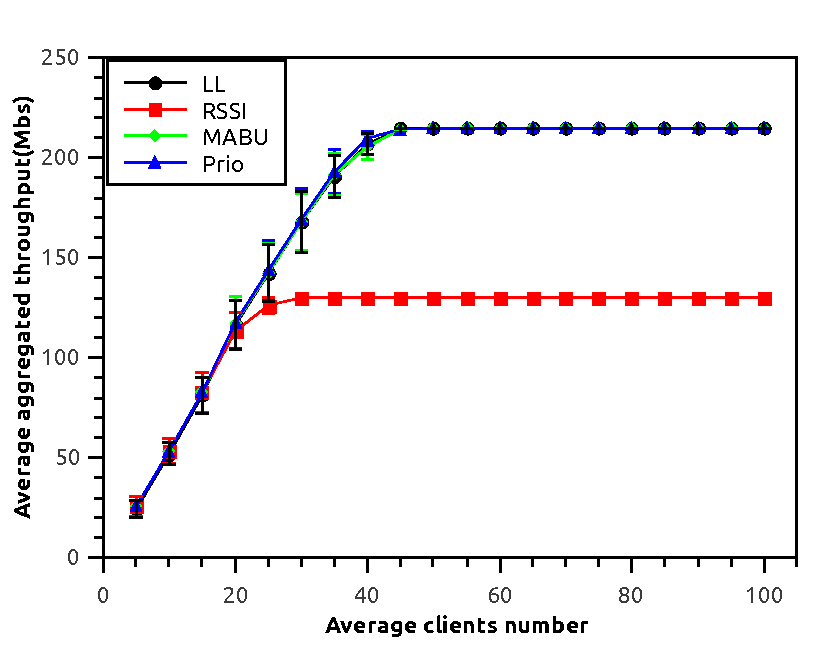
\includegraphics[scale=0.25]{Figures/offline/fix/v1/throughput/Graph-throughput.pdf}}
\hfil \subfigure[Average Aggregated throughput for classe 1 clients]{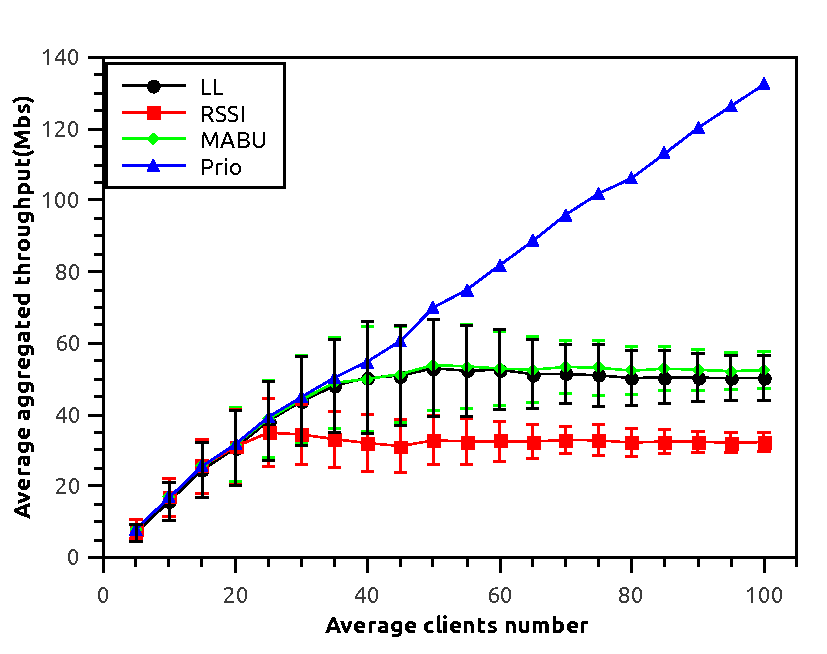
\includegraphics[scale=0.25]{Figures/offline/fix/v1/throughput/Graph-throughput-c1}}
\subfigure[Average Aggregated throughput for classe 2 clients]{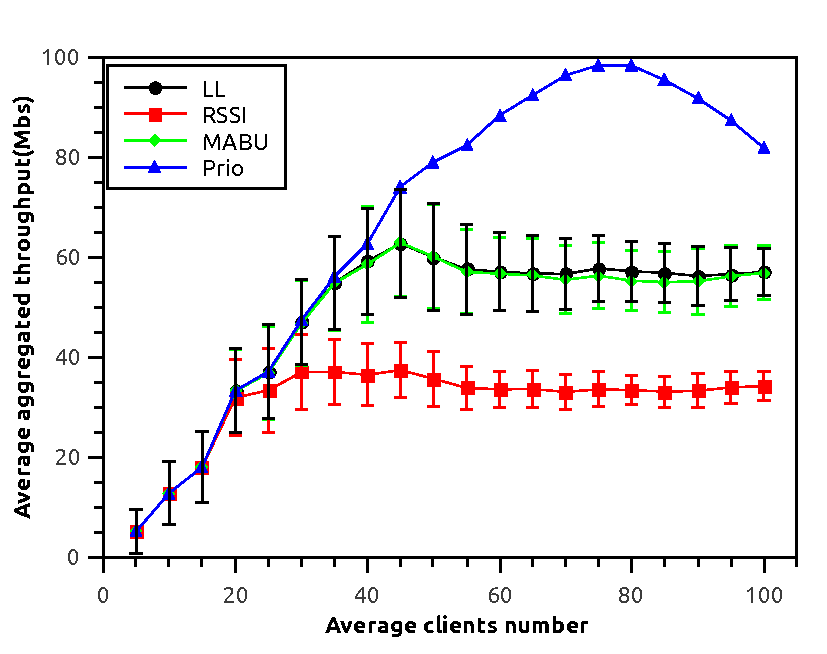
\includegraphics[scale=0.25]{Figures/offline/fix/v1/throughput/Graph-throughput-c2}}
\hfil \subfigure[Average Aggregated throughput for classe 3 clients]{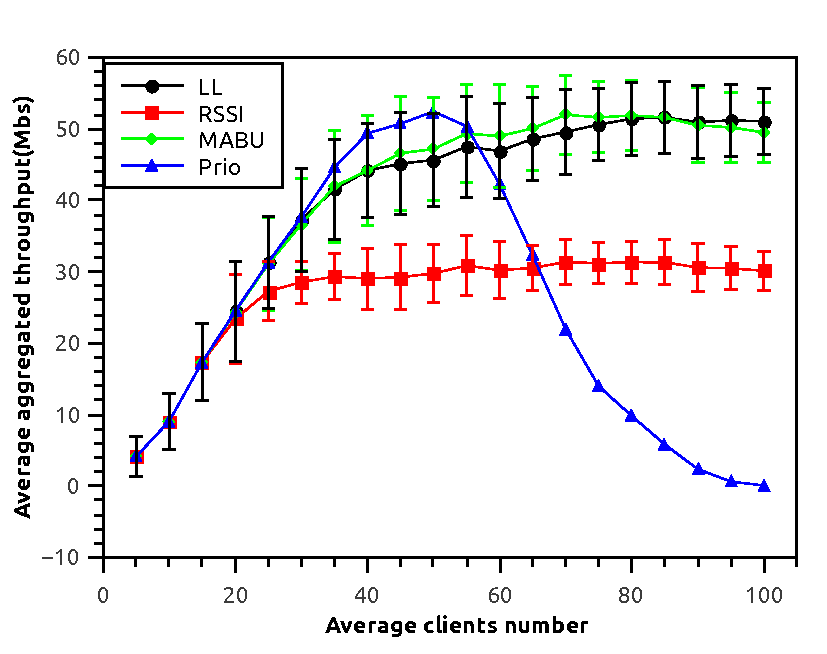
\includegraphics[scale=0.25]{Figures/offline/fix/v1/throughput/Graph-throughput-c3}}
\hfil \subfigure[Average Aggregated throughput for classe 4 clients]{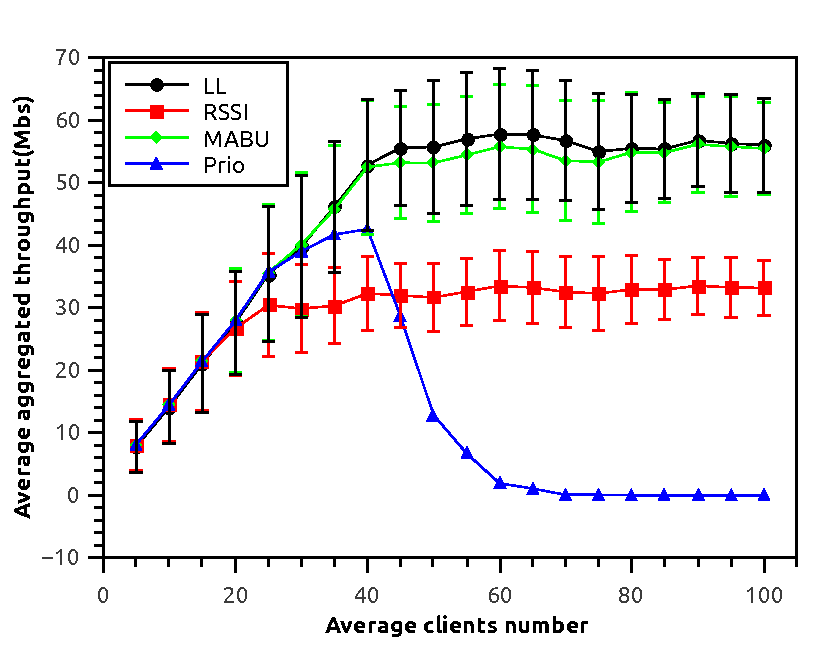
\includegraphics[scale=0.25]{Figures/offline/fix/v1/throughput/Graph-throughput-c4}}
\caption{Results for offline fix throughput}
\label{fig:results_offline_fix_throughput_v1} 
\end{figure*}

%===========================================================
%=====deficit   V1============
\begin{figure*}[t!]
\centering \subfigure[Average Aggregated deficit for all clients]{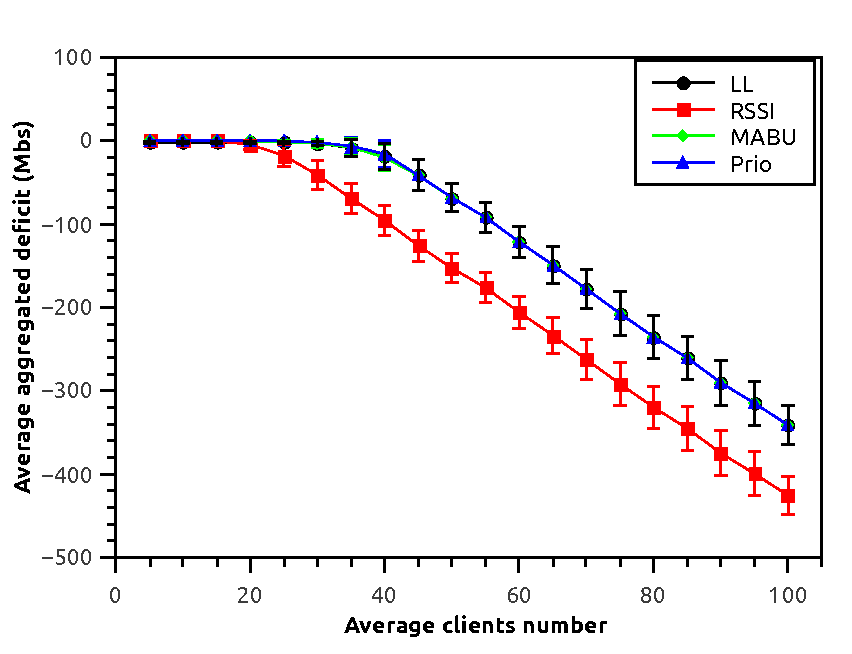
\includegraphics[scale=0.24]{Figures/offline/fix/v1/deficit/Graph-deficit.pdf}}
\hfil \subfigure[Average Aggregated deficit for classe 1 clients]{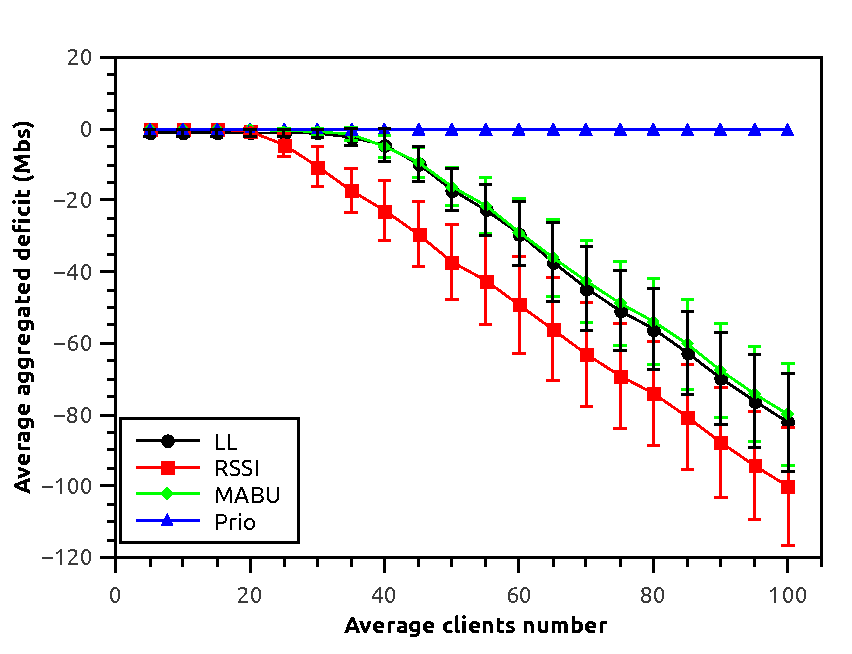
\includegraphics[scale=0.24]{Figures/offline/fix/v1/deficit/Graph-deficit-c1}}
\subfigure[Average Aggregated deficit for classe 2 clients]{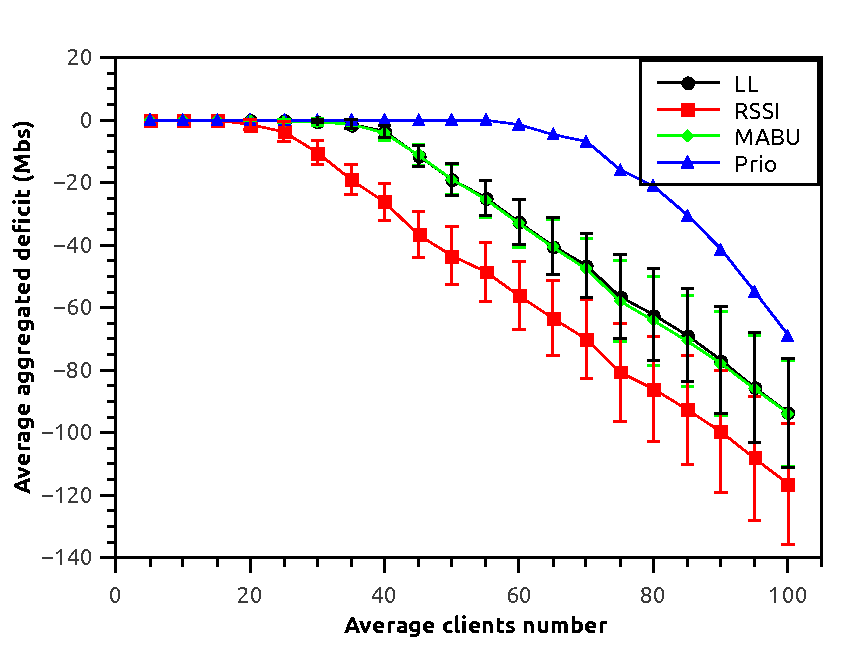
\includegraphics[scale=0.24]{Figures/offline/fix/v1/deficit/Graph-deficit-c2}}'
\hfil \subfigure[Average Aggregated deficit for classe 3 clients]{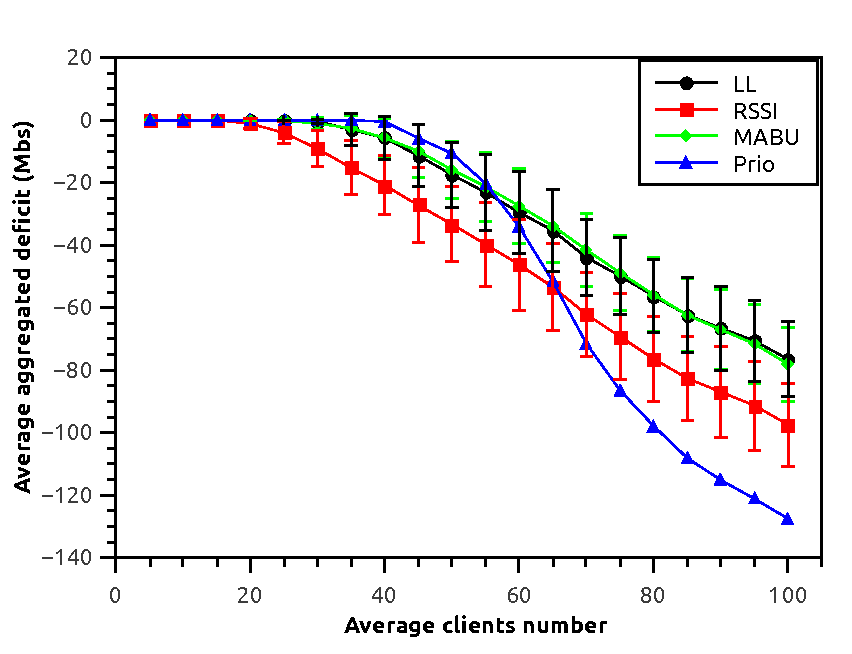
\includegraphics[scale=0.24]{Figures/offline/fix/v1/deficit/Graph-deficit-c3}}
\hfil \subfigure[Average Aggregated deficit for classe 4 clients]{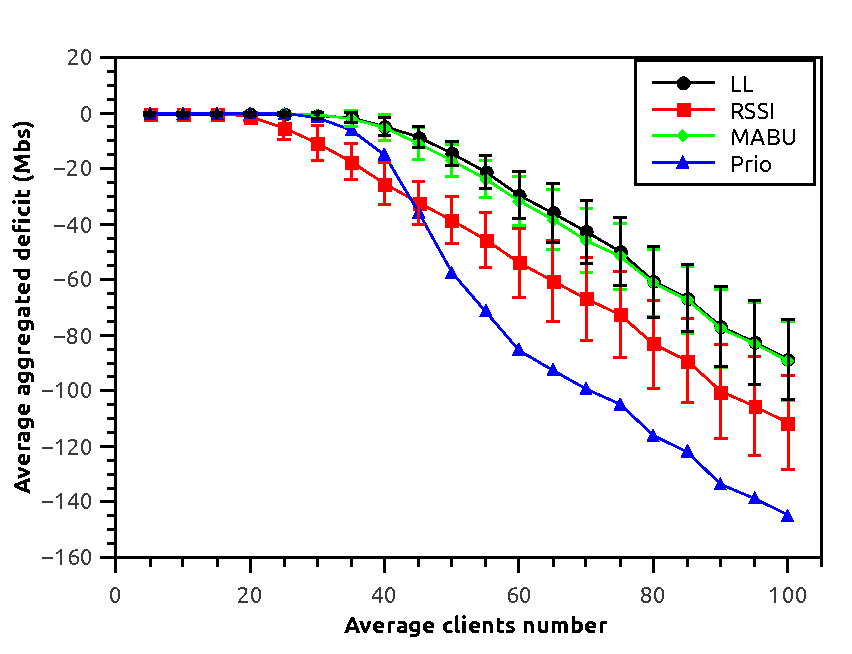
\includegraphics[scale=0.24]{Figures/offline/fix/v1/deficit/Graph-deficit-c4}}
\caption{Results for offline fix deficit}
\label{fig:results_offline_fix_deficit_v1} 
\end{figure*}

%===========================================================

%=====Nb Clients  deficit   V1============
\begin{figure*}[t!]
\centering \subfigure[Average Aggregated Nb clients in deficit for all clients]{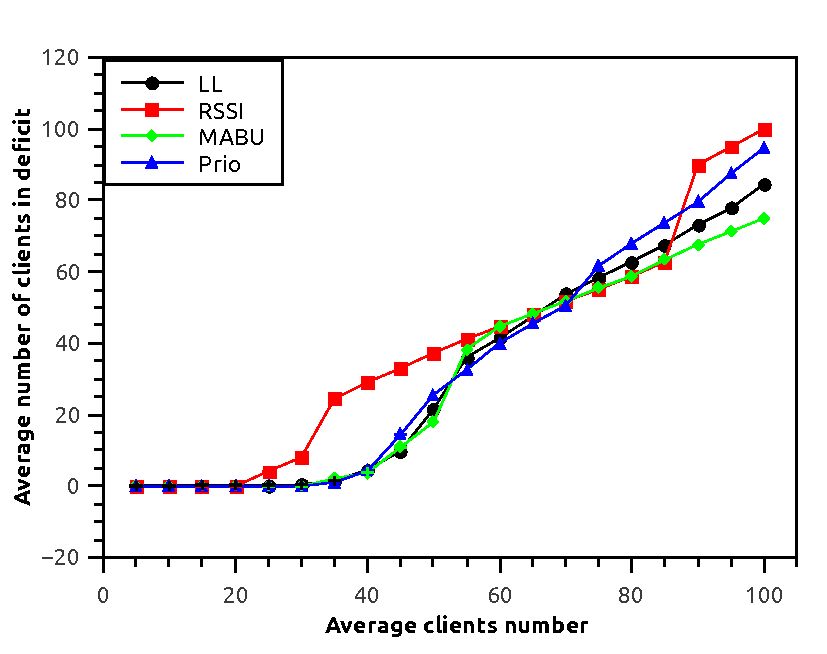
\includegraphics[scale=0.24]{Figures/offline/fix/v1/nb_deficit/Graph-nb-deficit.pdf}}
\hfil \subfigure[Average Aggregated Nb clients in deficit for classe 1 clients]{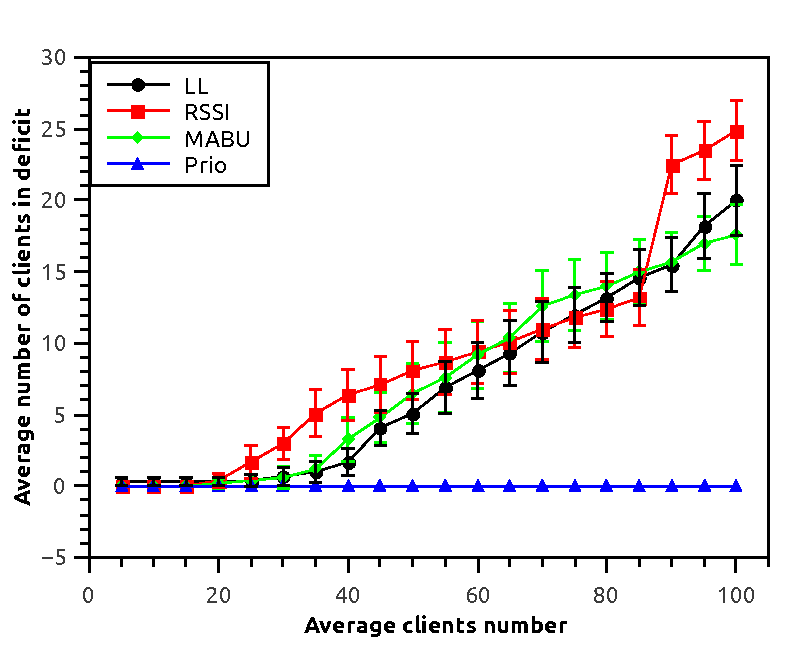
\includegraphics[scale=0.24]{Figures/offline/fix/v1/nb_deficit/Graph-nb-deficit-c1}}
\subfigure[Average Aggregated Nb clients in deficit for classe 2 clients]{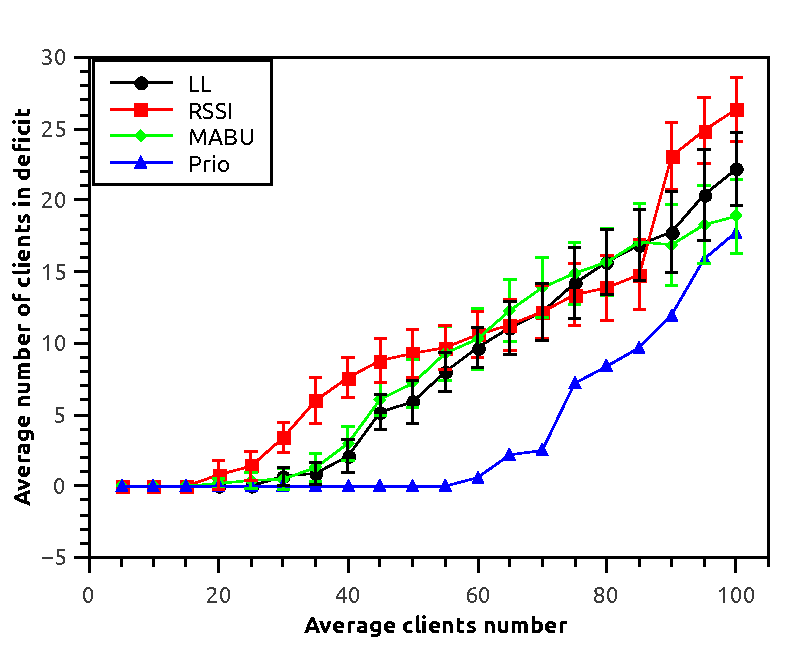
\includegraphics[scale=0.24]{Figures/offline/fix/v1/nb_deficit/Graph-nb-deficit-c2}}'
\hfil \subfigure[Average Aggregated Nb clients in deficit for classe 3 clients]{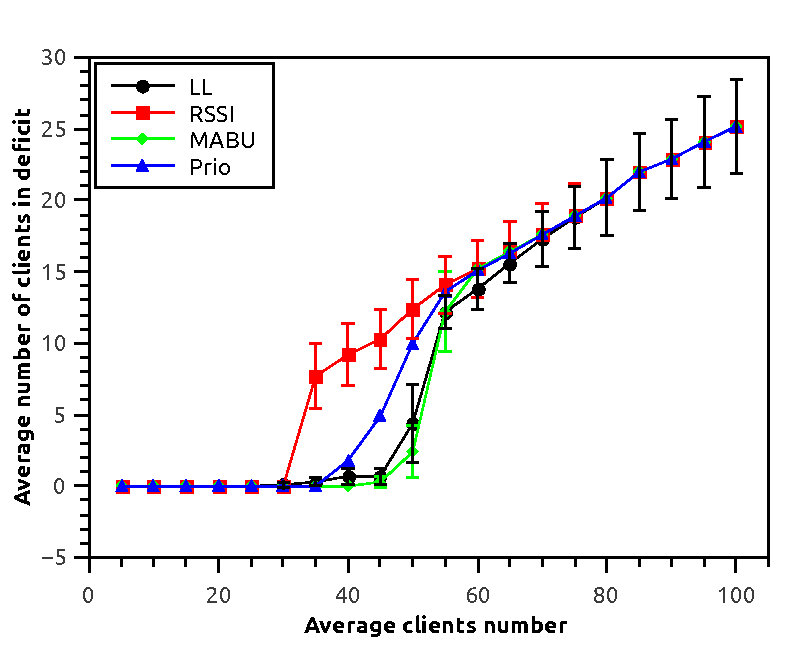
\includegraphics[scale=0.24]{Figures/offline/fix/v1/nb_deficit/Graph-nb-deficit-c3}}
\hfil \subfigure[Average Aggregated Nb clients in deficit for classe 4 clients]{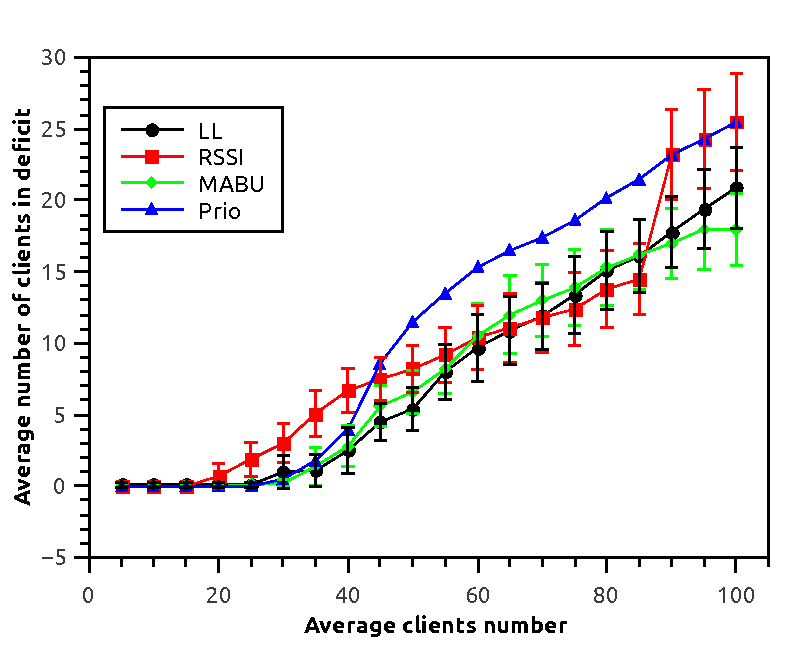
\includegraphics[scale=0.24]{Figures/offline/fix/v1/nb_deficit/Graph-nb-deficit-c4}}
\caption{Results for offline fix Nb clients in deficit}
\label{fig:results_offline_fix_Nb_clients_deficit_v1} 
\end{figure*}

%===========================================================

%=====APs Max and std loads V1 ============
\begin{figure}[t!]
\centering \subfigure[Average Max APs loads]{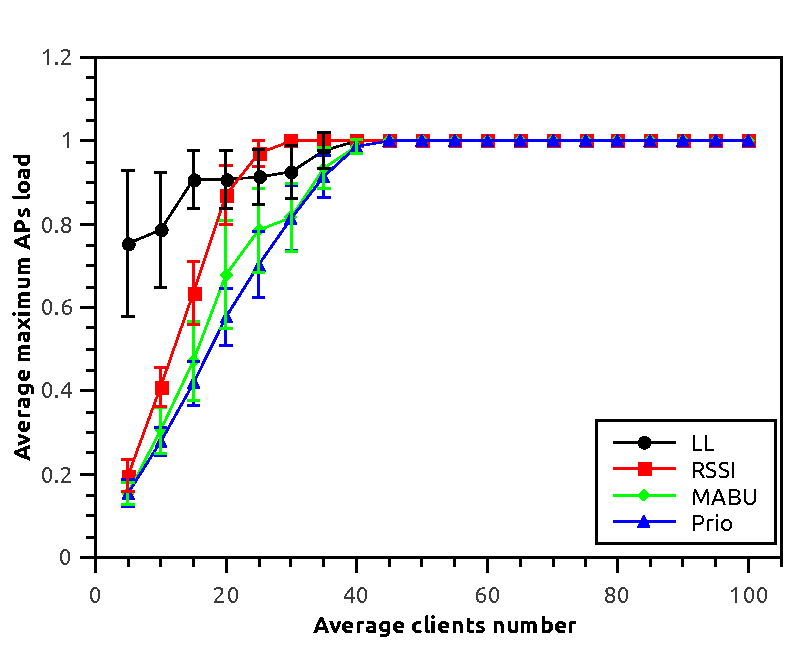
\includegraphics[scale=0.31]{Figures/offline/fix/v1/Graph-max-load.pdf}}
\subfigure[Average STD APs loads]{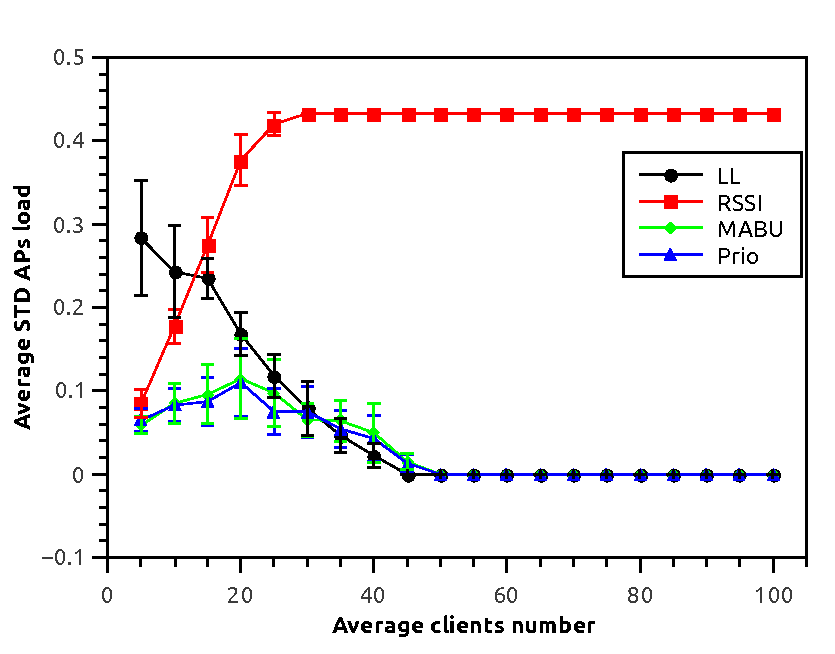
\includegraphics[scale=0.31]{Figures/offline/fix/v1/Graph-std-load.pdf}}
\caption{Results for offline fix APS MAX and STD loads}
\label{fig:results_offline_fix_loads} 
\end{figure}
%===========================================================
%========================================================= 

In our analysis, we interest specially to the downlink traffic that dominate the WLAN applications. We gave to each client a priority that corresponds in real applications to the importance of the work for the company. As explained in the previous sections, an example scenario that motivates this use (the project under which this work is made) is a cars showroom company in which the invitees have less priority that corresponds to the higher value 4. The company's staff those perform works from the second degree correspond to the priority 3. The priority of value 2 is given to the responsibles of the company, with any work to perform. The high priority that corresponds to value 1 is given to the technical staff at the moment of changing the version of cars software using diagnostic bags.
We have supposed in our evaluations two cases related to the clients priorities and demands. In the first one the high clients priorities do not necessarily correspond to the high capacity demands that take values in the set $\mathscr{D}=\left\{1.5, 5, 10 \right\}$ and are so chosen randomly. While in the second case the priority levels $\mathscr{P}=\left\{ 1,2,3,4\right\}$ correspond respectively to the demands 10, 5, 5, 1.5. In practice, the capacity demands are related to the chosen applications requirements that the clients are supposed to run such as video streaming, web-mail, file downloading...
In the online scenario, the users arrivals and departures are performed during the network lifetime. For that, we suppose that the arrivals follow Poisson law and the clients stay period in the network follows exponential distribution. On the other hand, for the offline evaluation, the users are supposed arriving at the beginning of the network lifetime. In order to evaluate the scheme scalability, the parameters are tunned to have an average number of clients in the system from 5 to 100. The duration of online simulation is 100000 seconds, while the offline one is immediate, as we just associate the clients with the Access Points with the envisaged capacity. 
Also from a point of uniformity distribution or dense network use, we have performed two scenarios. In the first one, the clients choose randomly their link capacities with the 4 Access Points at each arriving moment in the online scheme (or at the beginning of the network management for the offline version), in addition to the priorities and capacities demands. While in the second scenario, the clients distribution is not uniform and the first Access Point is supposed having the better link capacity of 130 Mbs with each client $i$ to emulate that the clients are closer to it, and the other three Access Points have respectively 52,26,6.5 Mbs. This configuration is frequent in real dense cellular WLAN, like that of train stations or airport gates, conferences rooms or malls' restaurants.   
In order to show the adequateness of our scheme, many candidates are used in both the offline and online scenarios evaluations. The standard Received Signal Strength Indicator based association (RSSI) could be applied to the two versions, in addition to that of the Least Loaded Access Points (LL) \cite{15dynamic_AP_association_SDN}. While MABU version \cite{16throughput_optimisation_association_bandwidth} is used as a third candidate in the offline version and Fitigness Factor (FF) \cite{17QOS_AP_selection} algorithm is used for the online scheme. 
For space constraints, we will show only the results corresponding to the random priorities and demands, and omit the version in which the priorities correspond to the capacity demands. So, we will have for the offline version two scenarios, one with the random uniform clients distribution and a second unbalanced with fixed capacities clients with the Access Points. The same scenarios are applied for the online scheme and so a uniform scenario with random clients deployment is applied in a first scenario, and a second scenario with fixed clients capacities with the Access Points is also performed.  

\subsection{Evaluation Metrics}
In order to quantify the previous evaluation scenarios results and show the superiority of the online and offline schemes, many metrics were chosen for comparison with other candidates. In the following a description of the chosen metrics:
 
\subsubsection{Average Aggregated throughput per priority level}
It is the sum of the amount of data received per second by the users of each priority level. Aggregated throughput value considers the sum of all the priority classes clients throughputs. As the aggregated throughput value is high as the indication of the global scheme good performance. But unfortunately, this metric does not highlight any fairness nor individual clients satisfaction.  

\subsubsection{Average Aggregated user deficit per priority level}
It is the sum of the difference between the given capacity for each client and its capacity demand according to each priority class. The aggregated deficit of all the network considers the average of the sum of all the priority classes clients deficits. As said for the previous metric, small values for this metric are good indication of the scheme adequateness, but does not reflect any fairness nor individual satisfaction. 
 
\subsubsection{Average number of clients in deficit per priority level}
This metric counts for the number of clients those are not satisfied because their affected capacities are less than their capacities demands per priority level. The aggregated number of clients in deficit quantifies all the clients of all the priority levels. The interpretation of this metric should be performed with that of the load of the Access points as explained in the following metric. But having a small value of this metric compared to the total number of clients in the system means that generally the clients are satisfied.  

\subsubsection{Average maximum APs load}
It is calculated as the average of the maximum APs load value seen at each second of the simulation. 
This metric should be interpreted with the previous and the next metrics together. Having a high value for this metric means that at least one Access Point is loaded and may be caused by a bad balancing of the Access Points load charges.

\subsubsection{Standard deviation of APs load}
This metric quantifies the charge balancing between the Access Points, as a small value of the load  standard deviation means that all the Access Points are equally loaded, while a high value means that the Access Points are not loaded fairly. Having a small value of the standard deviation in addition to a high value of the maximum Access Points load means that all the network is loaded and the number of clients in deficit will also be more significant.

%=========================================================

%==========offline  random figures==================================

%=====througput   V1============
\begin{figure*}[t!]
\centering \subfigure[Average Aggregated throughput for all clients]{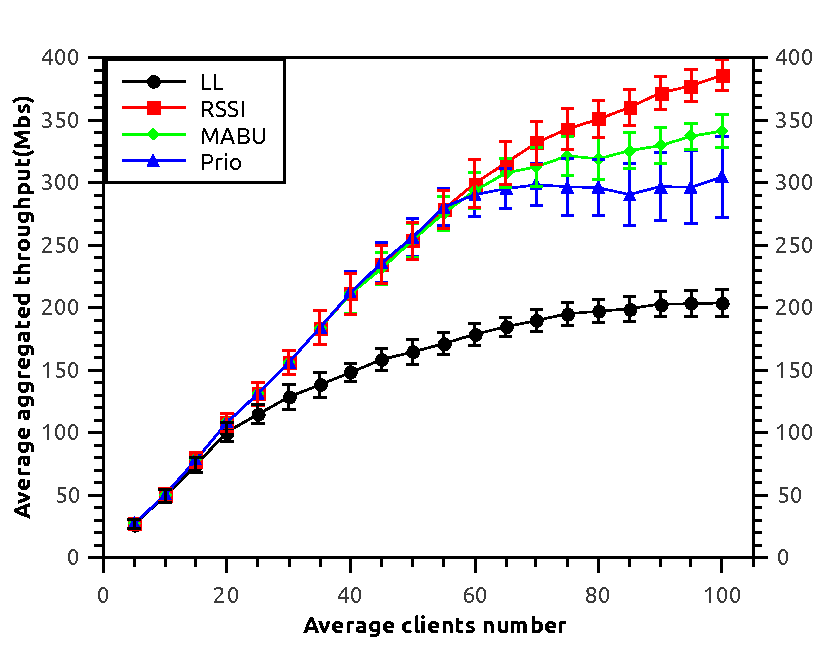
\includegraphics[scale=0.25]{Figures/offline/random_dem_var/v1/throughput/Graphe-throughput.pdf}}
\hfil \subfigure[Average Aggregated throughput for classe 1 clients]{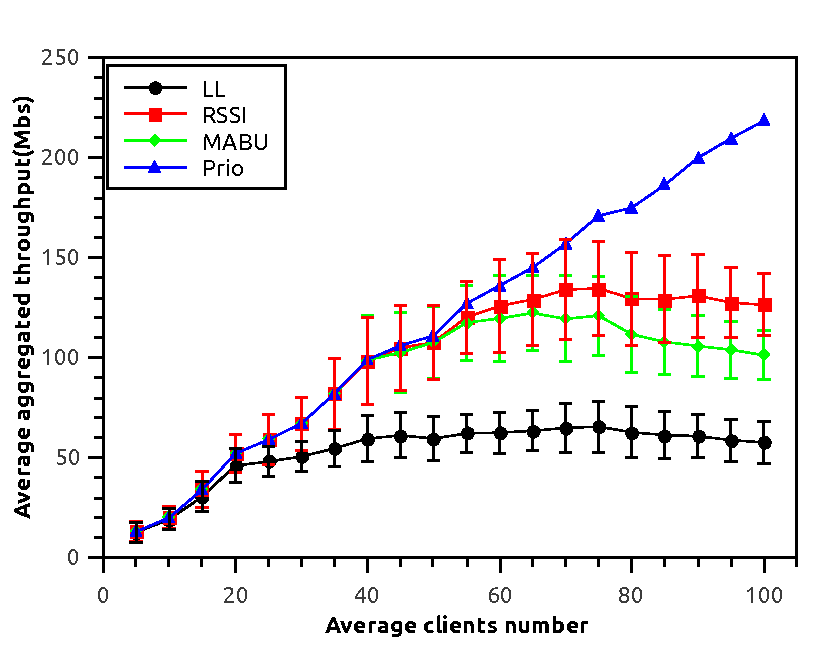
\includegraphics[scale=0.25]{Figures/offline/random_dem_var/v1/throughput/Graphe-throughput-c1}}
\subfigure[Average Aggregated throughput for classe 2 clients]{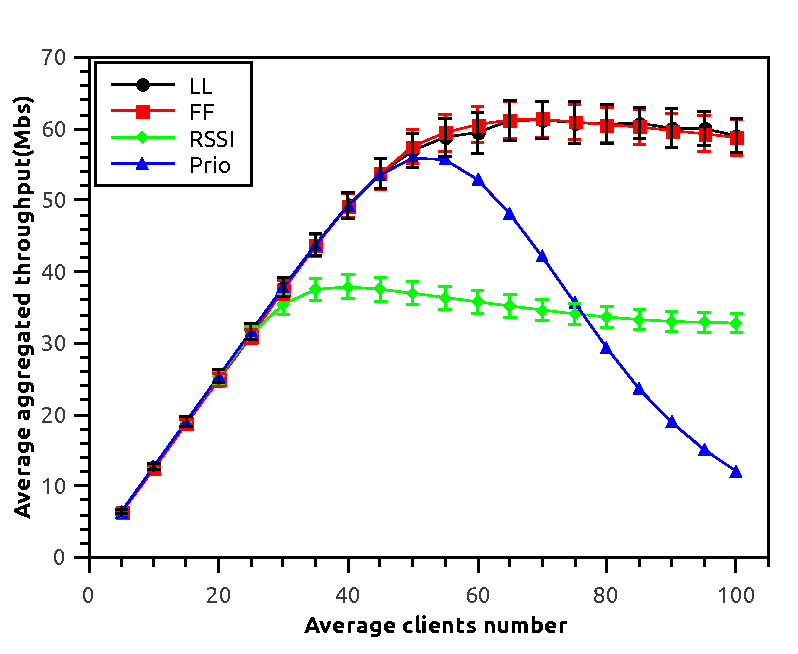
\includegraphics[scale=0.25]{Figures/offline/random_dem_var/v1/throughput/Graphe-throughput-c2}}
\hfil \subfigure[Average Aggregated throughput for classe 3 clients]{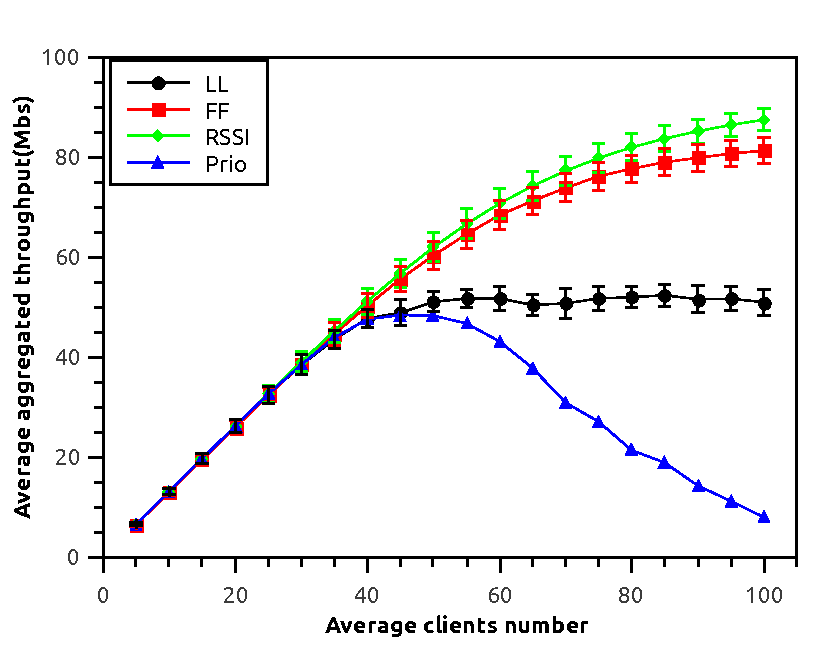
\includegraphics[scale=0.25]{Figures/offline/random_dem_var/v1/throughput/Graphe-throughput-c3}}
\hfil \subfigure[Average Aggregated throughput for classe 4 clients]{\includegraphics[scale=0.25]{Figures/offline/random_dem_var/v1/throughput/Graphe-throughput-c4}}
\caption{Results for offline random throughput}
\label{fig:results_offline_random_throughput_v1} 
\end{figure*}

%===========================================================

%=====deficit   V1============
\begin{figure*}[t!]
\centering \subfigure[Average Aggregated deficit for all clients]{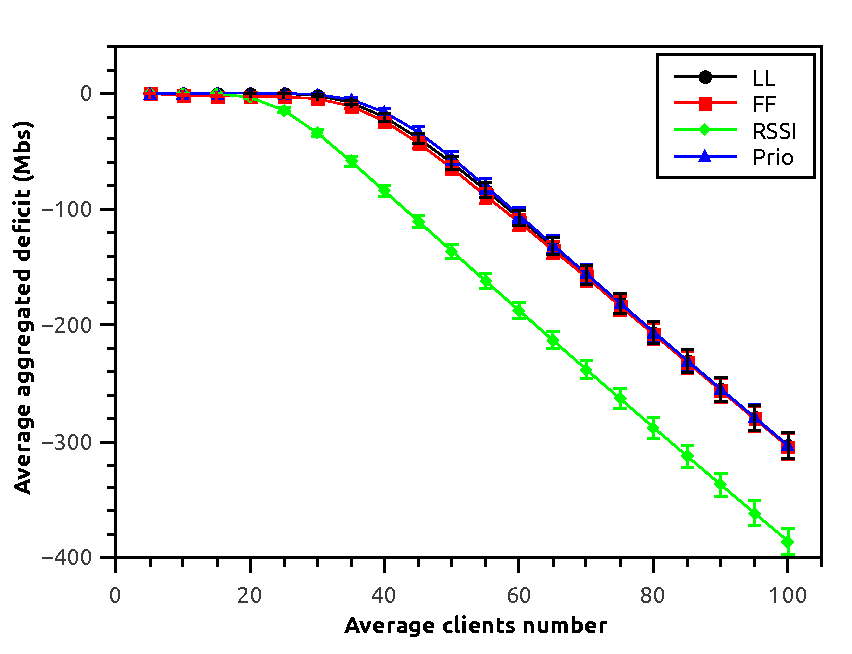
\includegraphics[scale=0.24]{Figures/offline/random_dem_var/v1/deficit/Graphe-deficit.pdf}}
\hfil \subfigure[Average Aggregated deficit for classe 1 clients]{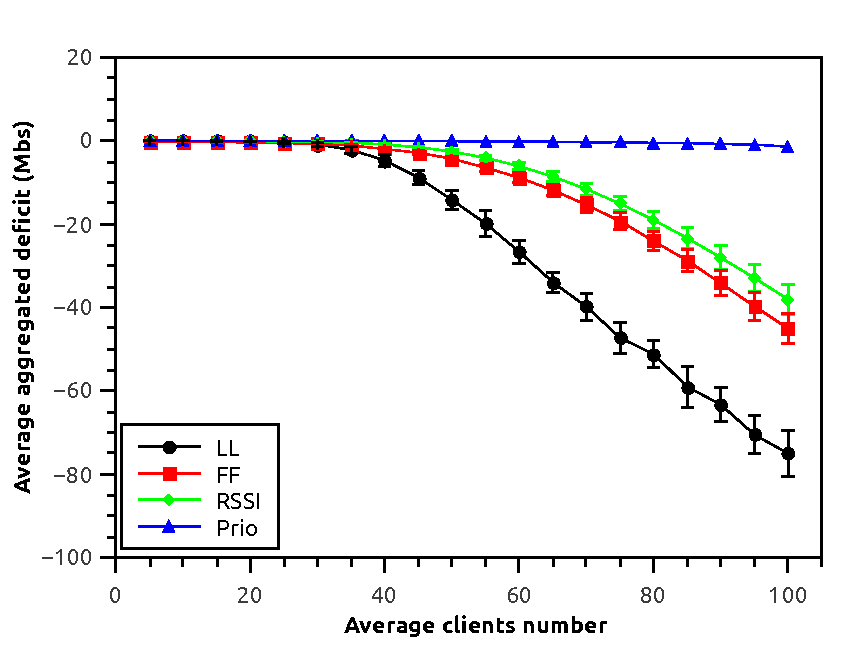
\includegraphics[scale=0.24]{Figures/offline/random_dem_var/v1/deficit/Graphe-deficit-c1}}
\subfigure[Average Aggregated deficit for classe 2 clients]{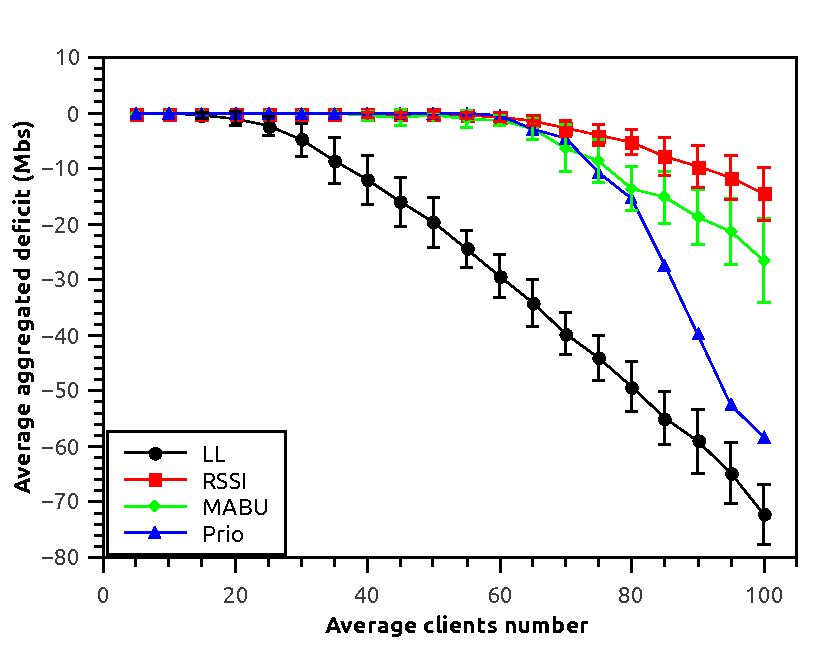
\includegraphics[scale=0.24]{Figures/offline/random_dem_var/v1/deficit/Graphe-deficit-c2}}'
\hfil \subfigure[Average Aggregated deficit for classe 3 clients]{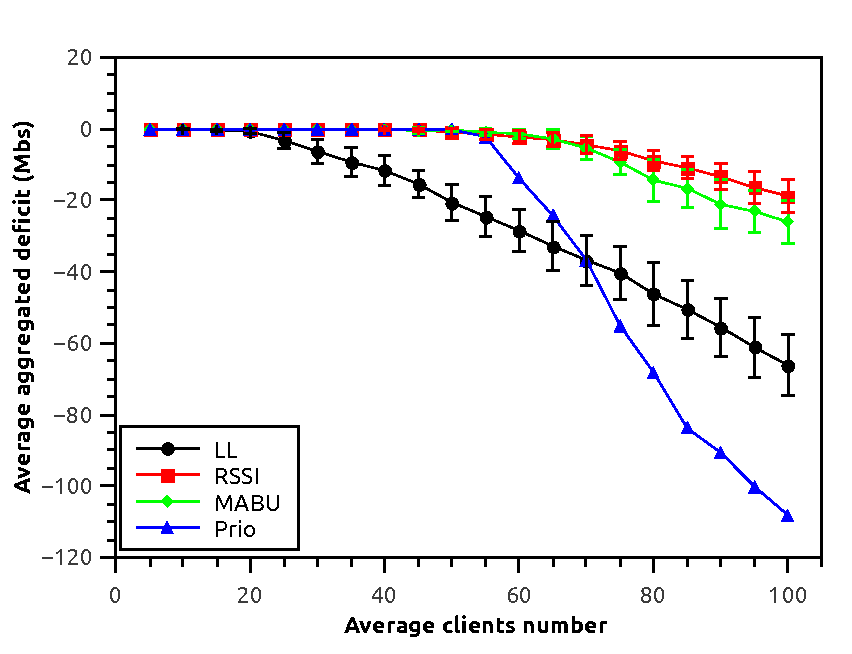
\includegraphics[scale=0.24]{Figures/offline/random_dem_var/v1/deficit/Graphe-deficit-c3}}
\hfil \subfigure[Average Aggregated deficit for classe 4 clients]{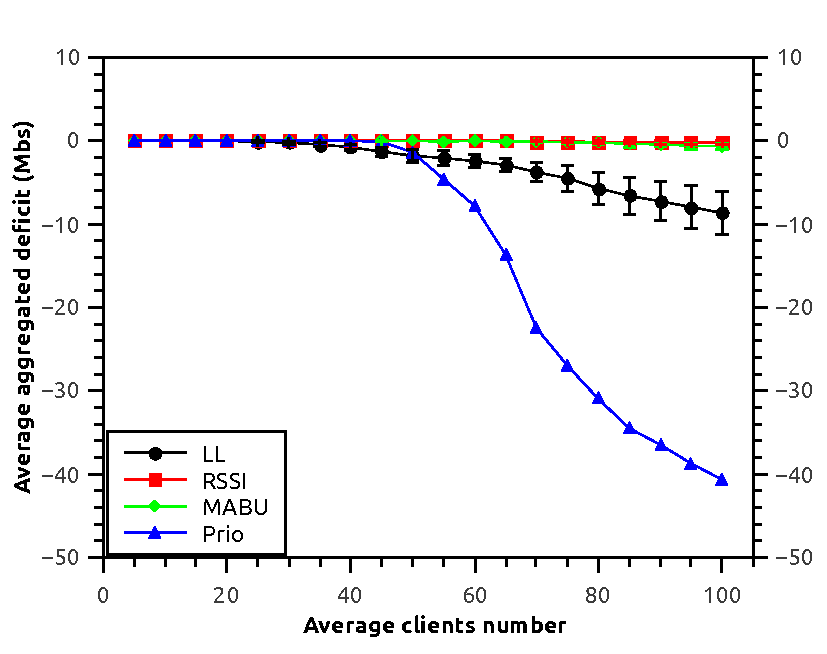
\includegraphics[scale=0.24]{Figures/offline/random_dem_var/v1/deficit/Graphe-deficit-c4}}
\caption{Results for offline random deficit}
\label{fig:results_offline_random_deficit_v1} 
\end{figure*}

%===========================================================

%=====Nb Clients  deficit   V1============
\begin{figure*}[t!]
\centering \subfigure[Average Aggregated Nb clients in deficit for all clients]{\includegraphics[scale=0.24]{Figures/offline/random_dem_var/v1/nb_deficit/Graphe-nb-deficit.pdf}}
\hfil \subfigure[Average Aggregated Nb clients in deficit for classe 1 clients]{\includegraphics[scale=0.24]{Figures/offline/random_dem_var/v1/nb_deficit/Graphe-nb-deficit-c1}}
\subfigure[Average Aggregated Nb clients in deficit for classe 2 clients]{\includegraphics[scale=0.24]{Figures/offline/random_dem_var/v1/nb_deficit/Graphe-nb-deficit-c2}}'
\hfil \subfigure[Average Aggregated Nb clients in deficit for classe 3 clients]{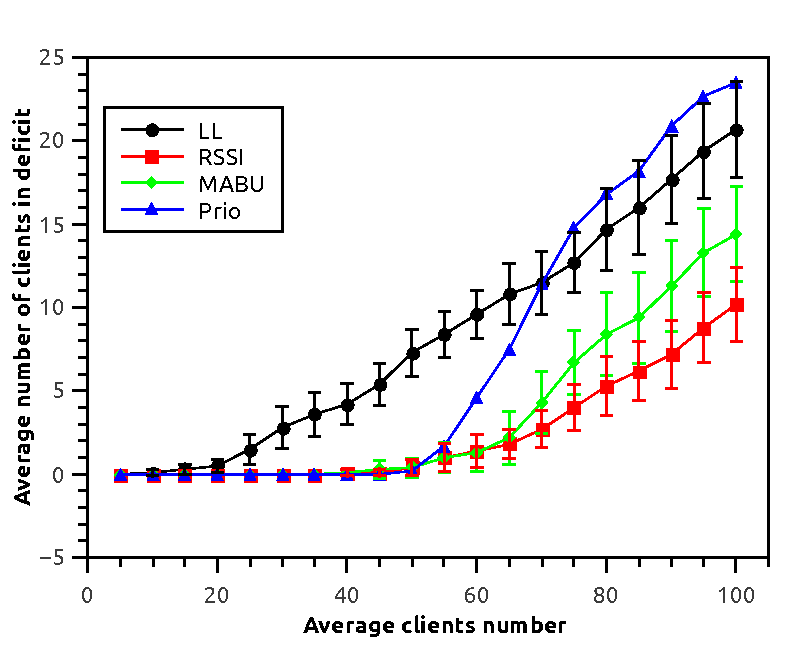
\includegraphics[scale=0.24]{Figures/offline/random_dem_var/v1/nb_deficit/Graphe-nb-deficit-c3}}
\hfil \subfigure[Average Aggregated Nb clients in deficit for classe 4 clients]{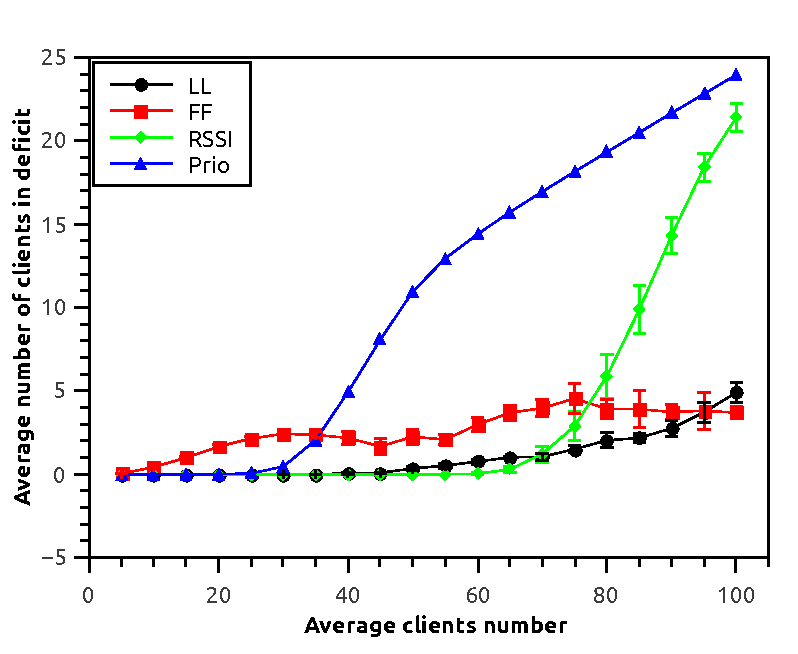
\includegraphics[scale=0.24]{Figures/offline/random_dem_var/v1/nb_deficit/Graphe-nb-deficit-c4}}
\caption{Results for offline random Nb clients in deficit}
\label{fig:results_offline_random_Nb_clients_deficit_v1} 
\end{figure*}

%===========================================================

%=====APs Max and std loads V1 ============
\begin{figure}[t!]
\centering \subfigure[Average Max APs loads]{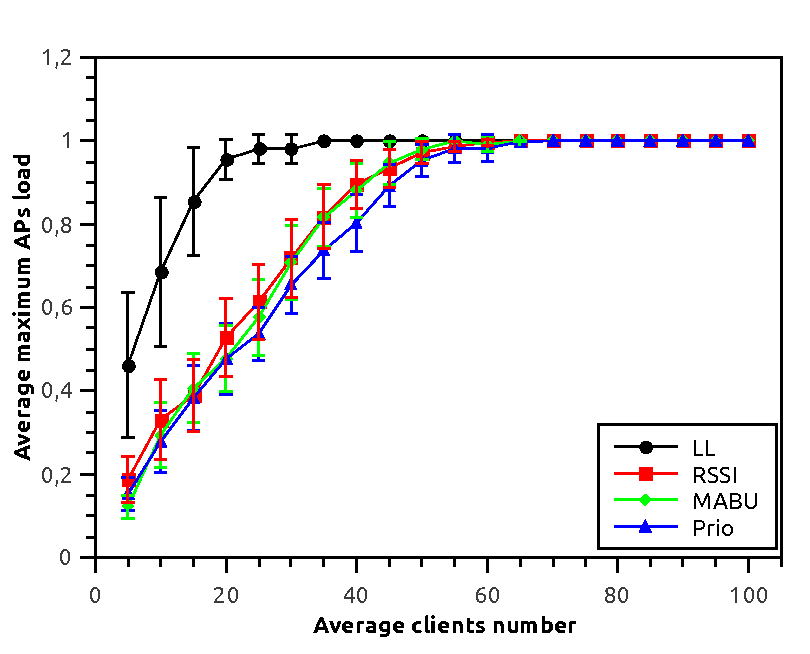
\includegraphics[scale=0.31]{Figures/offline/random_dem_var/v1/Graphe-max-load.pdf}}
\subfigure[Average STD APs loads]{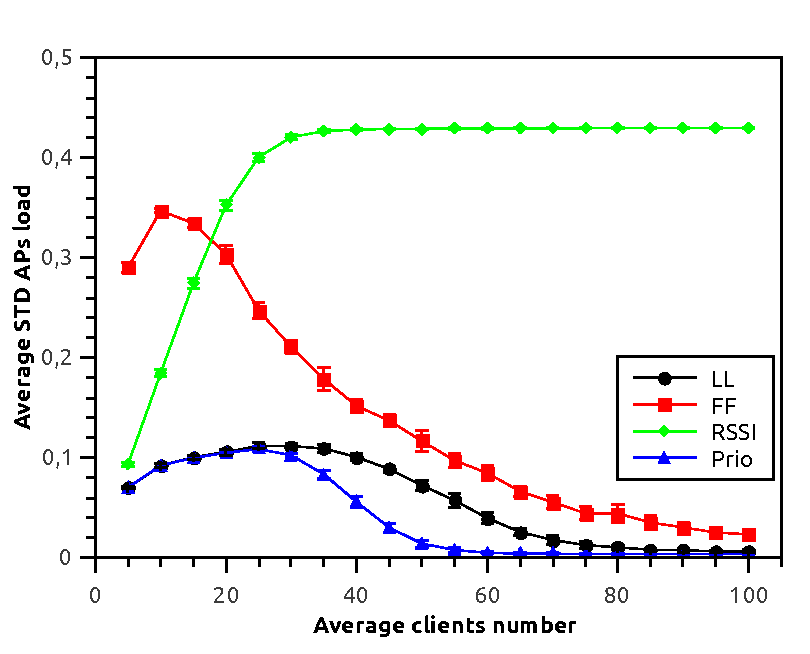
\includegraphics[scale=0.3]{Figures/offline/random_dem_var/v1/Graphe-std-load.pdf}}
\caption{Results for offline random positions APs MAX and STD loads}
\label{fig:results_offline_random_loads} 
\end{figure}

%=========================================================

\subsection{Evaluation results}

In this section we analyse and explain the simulation results for offline and online schemes for their fixed location and random location users scenarios.

\subsubsection{offline scheme evaluation}
As explained before, in this case, all the clients are supposed present at the beginning of the execution network.
\paragraph{Fixed location scenario} This scenario corresponds to the case that all the clients are concentrated in the vicinity of a given Access Point from the beginning of the network lifetime, that translates to a high capacity with it, in our scenario 130 Mbs as a link capacity and respectively 52,26,6.5 Mbs with the others. The standard IEEE association will associate all the clients with this Access Point leading to overloading of the strongest signal Access point, while the other candidates try to balance the clients thorough the other Access Points. The difference between our scheme (noted Prio, for priority handling) and the two other ones, namely MABU and Least loaded (LL) is that they don't give importance to the clients priorities and share the resources based on simple time fairness, while our scheme (Prio) starts by associating the clients in a balanced manner according to their high priorities, and just after give them as possible their required capacity demands in priority based max-min time fairness. As the Access Points have limited capacities, the low priority clients in our scheme could be associated without being given any capacity resources until the higher priority clients consume their capacity demands and free the channel resources. This is clearly seen in the Figure\ref{fig:results_offline_fix_throughput_v1}.a,b,c,d,e as the MABU and LL schemes in addition to the ours have a similar aggregated throughput (\ref{fig:results_offline_fix_throughput_v1}.a) which is clearly better than that of the standard RSSI based. But the clients with higher priority have more throughput than the less priority ones for our scheme, contrary to the other schemes for which the clients have strict time fairness according to their demands (\ref{fig:results_offline_fix_throughput_v1}.b,c,d,e). The same remark could be given to the Figure\ref{fig:results_offline_fix_deficit_v1}.a,b,c,d,e as the clients in the higher priority classes have less deficit than the less priority ones in our scheme, while the two other schemes treat the clients equally. The RSSI based scheme continues to have the important deficit as all the clients concentrate in the higher signal Access Point. In the Figure\ref{fig:results_offline_fix_Nb_clients_deficit_v1}.a,b,c,d,e the number of clients in deficit follows the priority classes for our scheme contrary to the other schemes that treat the clients equally without importance of priority, and the same remark continues with the RSSI based scheme with the higher number of clients in deficit. The Figure.\ref{fig:results_offline_fix_loads}.a,c confirms the load balancing of the Access points charges for the three schemes contrary to the RSSI based scheme, as the maximum load value becomes high for the three schemes in accordance with the standard deviation small value of the Access Points loads which confirms that all the Access Points become loaded starting from 40 clients in the network, while the RSSI based scheme loads only one Access Point with all the clients and keeps the other ones empty.   
   
\paragraph{Random location scenario}
Contrary to the previous scenario, in this one, the clients are randomly distributed in the network, having different link capacities with the Access Points. This is in favour of the RSSI based scheme as it can be shown in all the performance metrics. Indeed, having random capacities will load balance the load charge automatically for the RSSI based scheme. The MABU scheme also presents good performance as its load balancing scheme is well made. The LL scheme presents less performance compared to the two previous ones. Our scheme has better performance of aggregated throughput, deficit and number of clients with deficit than that of LL but less than that of RSSI and MABU. But as the Figure \ref{fig:results_offline_random_throughput_v1}.b,c, Figure\ref{fig:results_offline_random_deficit_v1}.b,c, and Figure\ref{fig:results_offline_random_Nb_clients_deficit_v1}.b,c show, our scheme gets better performance for higher priority clients, and less performance for the less priority clients. This can be explained that a higher priority client could have bad link capacity with all the Access Points, but should be given its bandwidth demand, which translates to monopolising all the channel until having its demand. This handicaps other clients with less priority associated with the same Access Points. But in practice, as motivated in our chosen real application, the technical staff must finish their work using their diagnostic bags before sharing the link resources of the Access Point equally with the other showroom invitees. Rather, the system version of the car modified with this technical operation risks to take very long time, which enhances the probability of system update failure. In Figure \ref{fig:results_offline_random_loads}.a,c the load balancing of all the schemes can be seen. Our scheme presents good results of balancing the clients. The LL scheme balancing method ensure very good balancing of the Access Points load charge. But the fact of doing this balancing load in a random order of clients service order in the global list showed that it does not automatically translates to a better throughput. At the contrary, the MABU scheme sorts the clients demands before starting the association, which gives less balancing but with better performance. As said before the RSSI scheme balances automatically the clients by the fact that are supposed having random capacities.      

%==========online  fix figures==================================

%=====througput   V1============
\begin{figure*}[t!]
\centering \subfigure[Average Aggregated throughput for all clients]{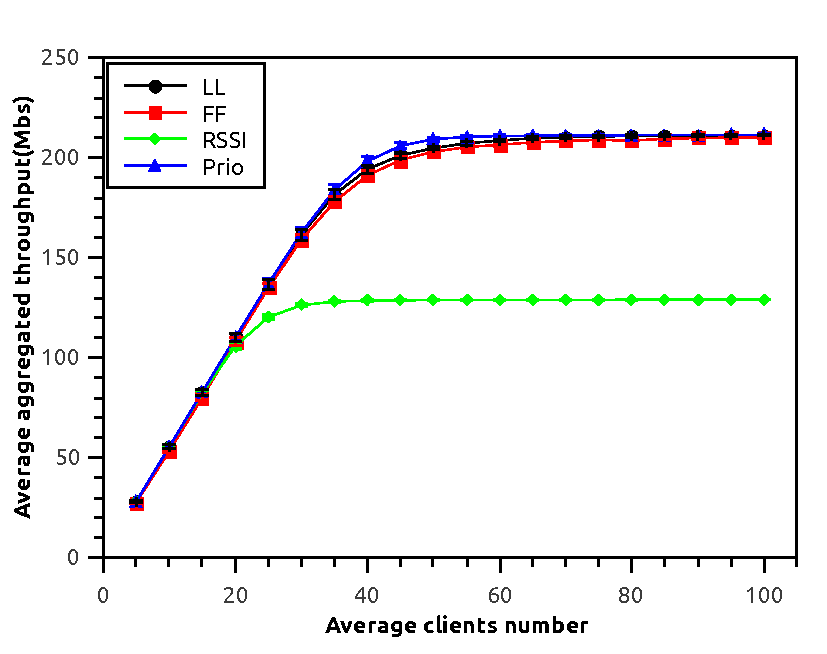
\includegraphics[scale=0.25]{Figures/online/fix/v1/throughput/Graphe-throughput-all.pdf}}
\hfil \subfigure[Average Aggregated throughput for classe 1 clients]{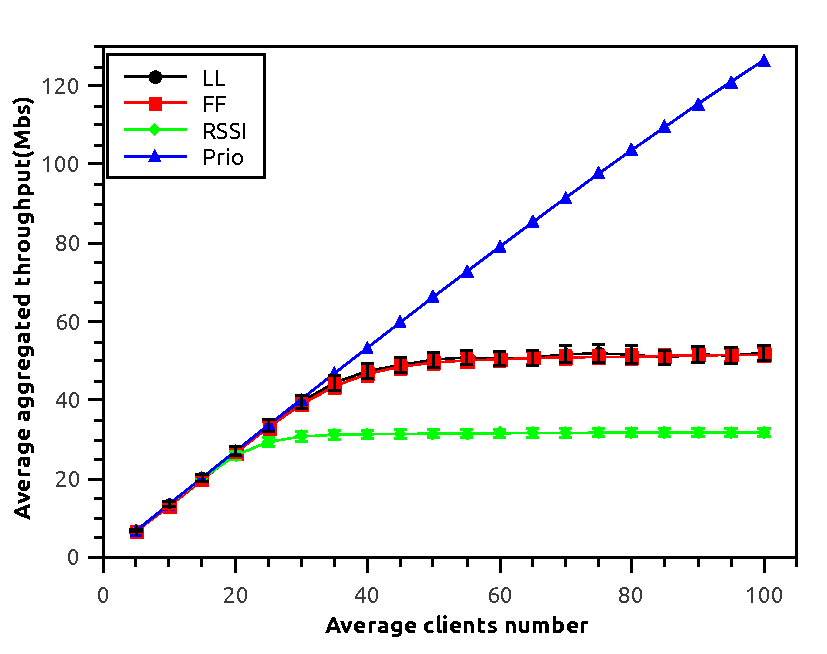
\includegraphics[scale=0.25]{Figures/online/fix/v1/throughput/Graphe-throughput-c1}}
\subfigure[Average Aggregated throughput for classe 2 clients]{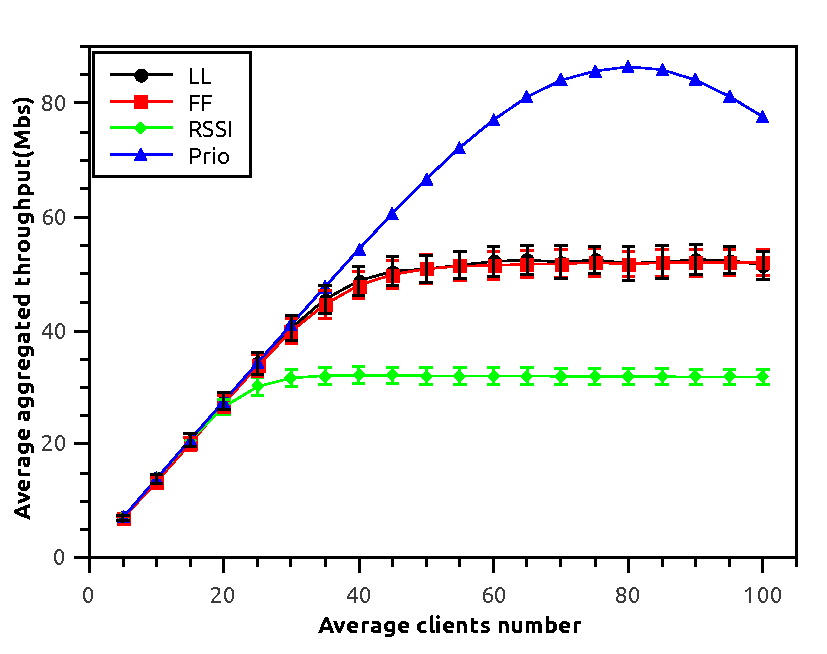
\includegraphics[scale=0.25]{Figures/online/fix/v1/throughput/Graphe-throughput-c2}}
\hfil \subfigure[Average Aggregated throughput for classe 3 clients]{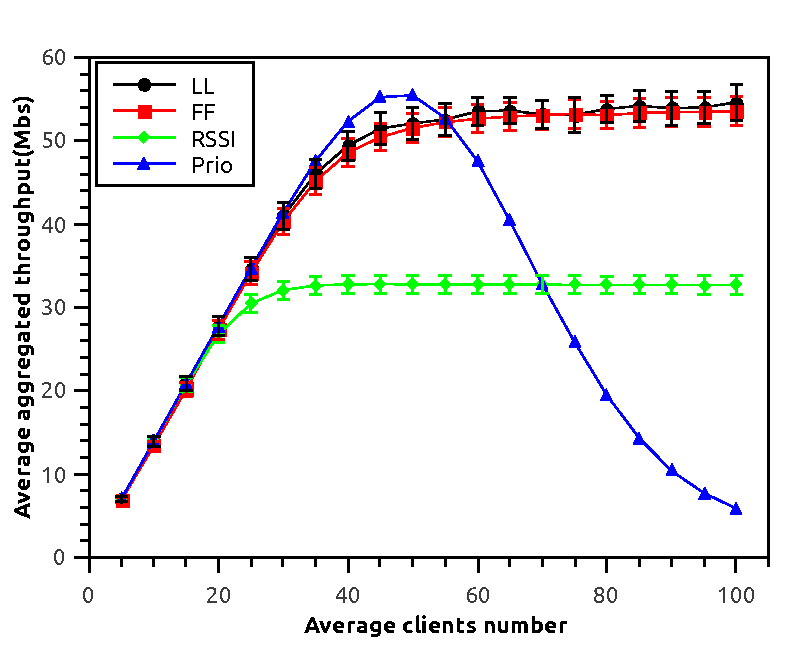
\includegraphics[scale=0.25]{Figures/online/fix/v1/throughput/Graphe-throughput-c3}}
\hfil \subfigure[Average Aggregated throughput for classe 4 clients]{\includegraphics[scale=0.25]{Figures/online/fix/v1/throughput/Graphe-throughput-c4}}
\caption{Results for online fix throughput}
\label{fig:results_online_fix_throughput_v1} 
\end{figure*}

%===========================================================

%=====deficit   V1============
\begin{figure*}[t!]
\centering \subfigure[Average Aggregated deficit for all clients]{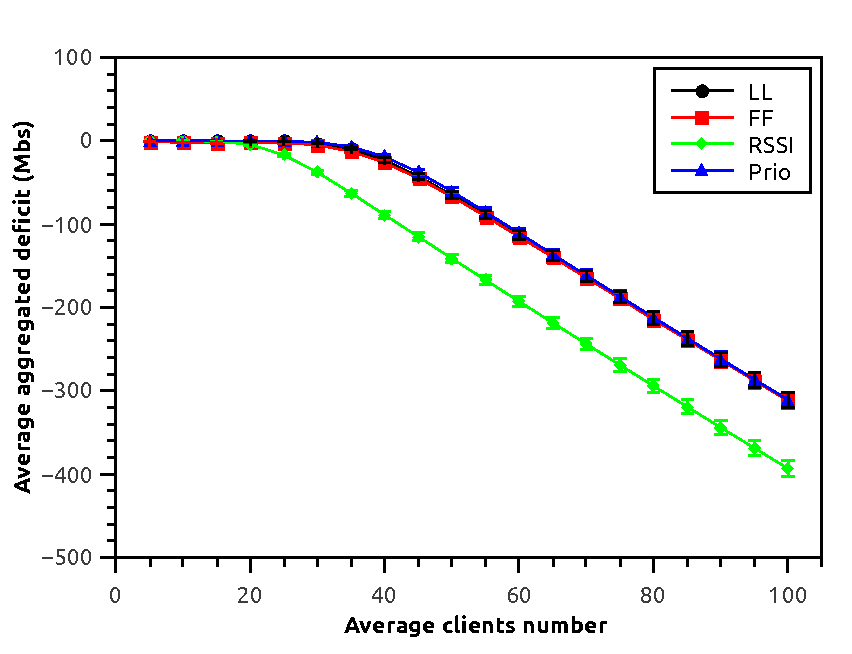
\includegraphics[scale=0.24]{Figures/online/fix/v1/deficit/Graph-deficit-all.pdf}}
\hfil \subfigure[Average Aggregated deficit for classe 1 clients]{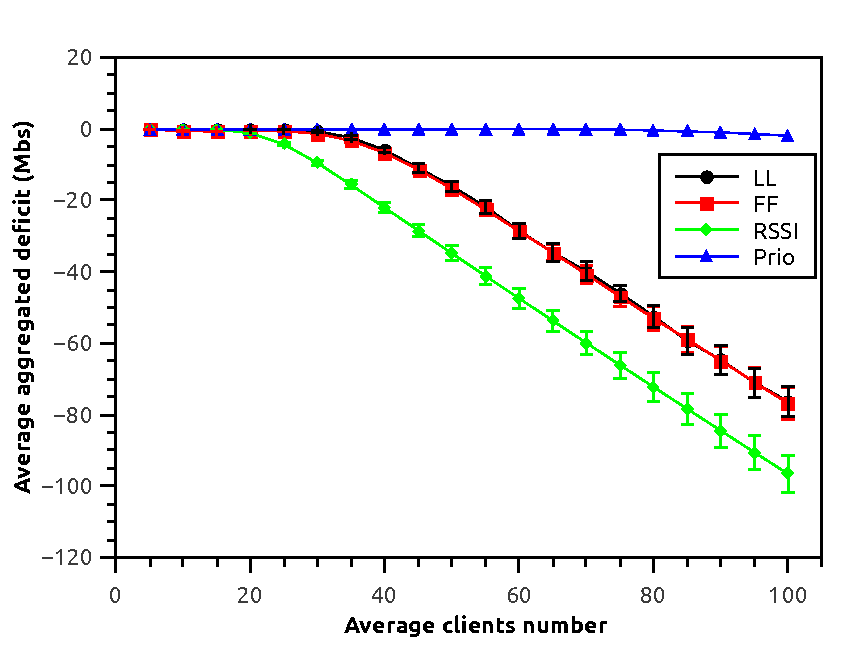
\includegraphics[scale=0.24]{Figures/online/fix/v1/deficit/Graph-deficit-c1}}
\subfigure[Average Aggregated deficit for classe 2 clients]{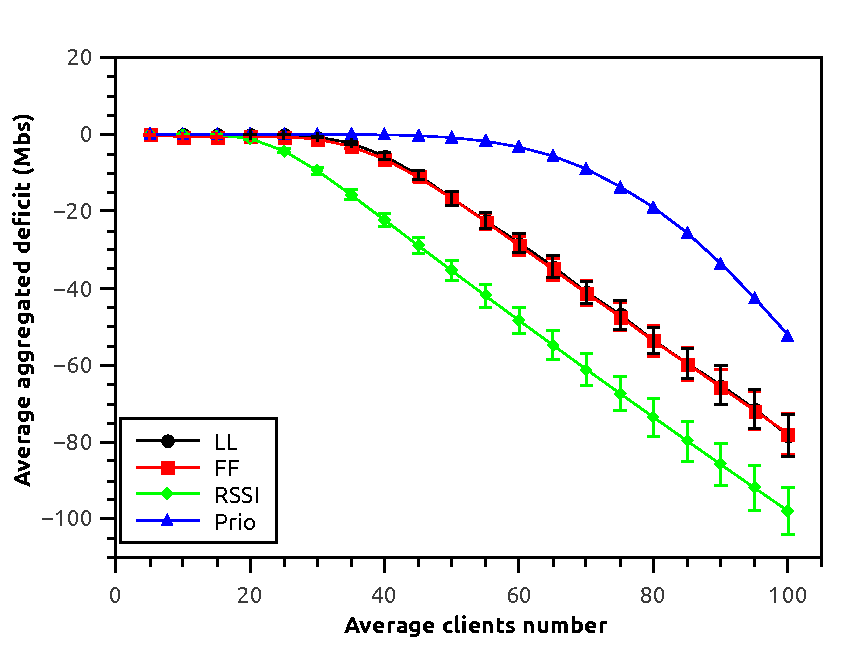
\includegraphics[scale=0.24]{Figures/online/fix/v1/deficit/Graph-deficit-c2}}'
\hfil \subfigure[Average Aggregated deficit for classe 3 clients]{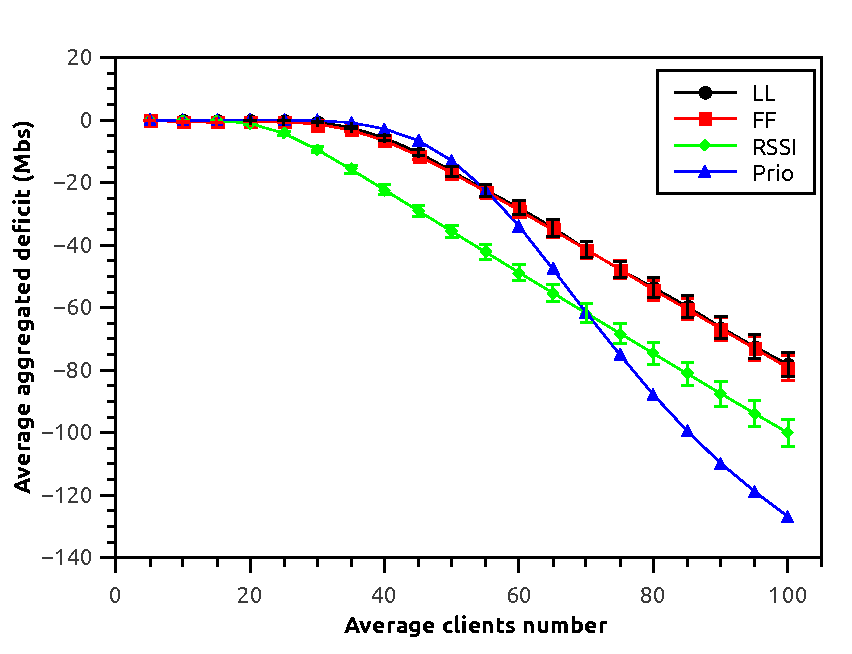
\includegraphics[scale=0.24]{Figures/online/fix/v1/deficit/Graph-deficit-c3}}
\hfil \subfigure[Average Aggregated deficit for classe 4 clients]{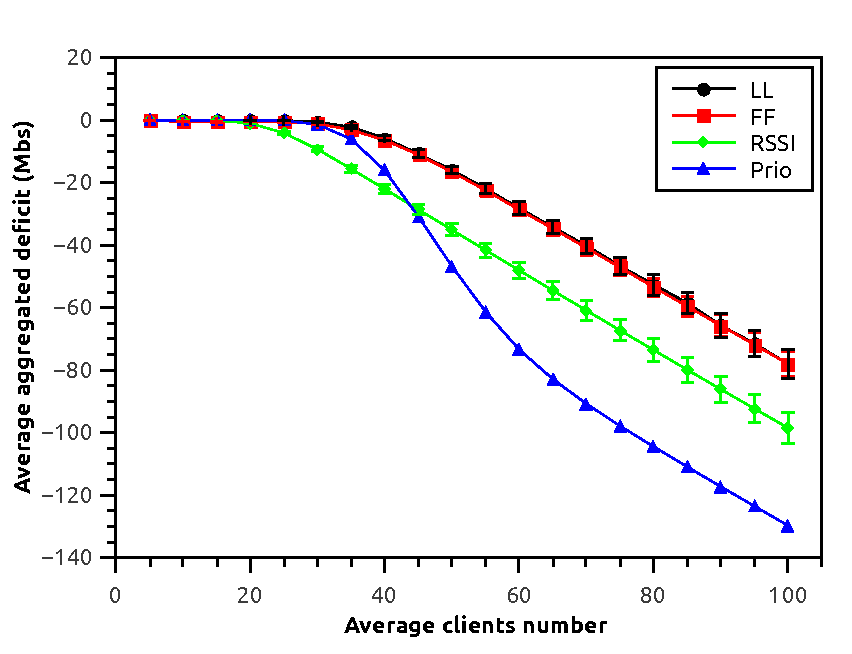
\includegraphics[scale=0.24]{Figures/online/fix/v1/deficit/Graph-deficit-c4}}
\caption{Results for online fix deficit}
\label{fig:results_online_fix_deficit_v1} 
\end{figure*}

%===========================================================

%=====Nb Clients  deficit   V1============
\begin{figure*}[t!]
\centering \subfigure[Average Aggregated Nb clients in deficit for all clients]{\includegraphics[scale=0.24]{Figures/online/fix/v1/nb_deficit/Graphe-nb-deficit.pdf}}
\hfil \subfigure[Average Aggregated Nb clients in deficit for classe 1 clients]{\includegraphics[scale=0.24]{Figures/online/fix/v1/nb_deficit/Graphe-nb-deficit-c1}}
\subfigure[Average Aggregated Nb clients in deficit for classe 2 clients]{\includegraphics[scale=0.24]{Figures/online/fix/v1/nb_deficit/Graphe-nb-deficit-c2}}'
\hfil \subfigure[Average Aggregated Nb clients in deficit for classe 3 clients]{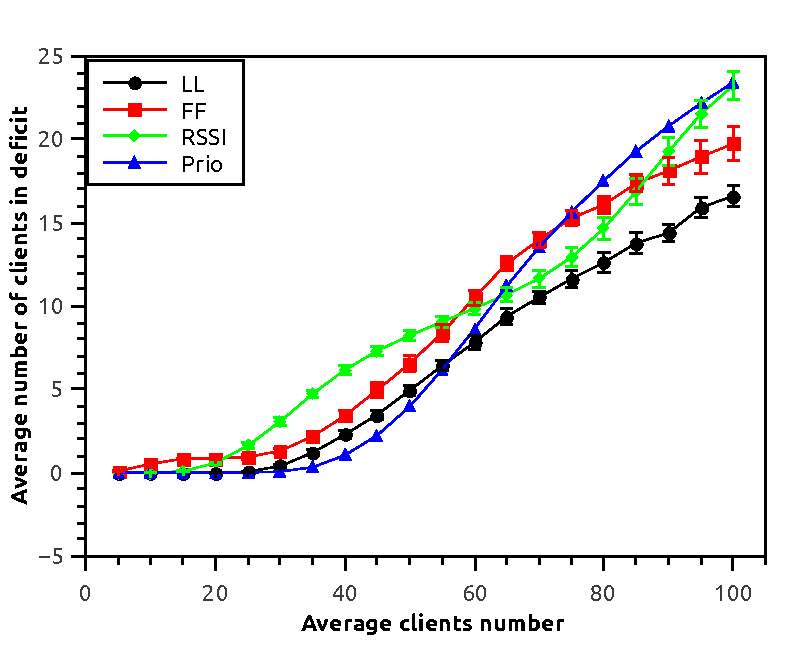
\includegraphics[scale=0.24]{Figures/online/fix/v1/nb_deficit/Graphe-nb-deficit-c3}}
\hfil \subfigure[Average Aggregated Nb clients in deficit for classe 4 clients]{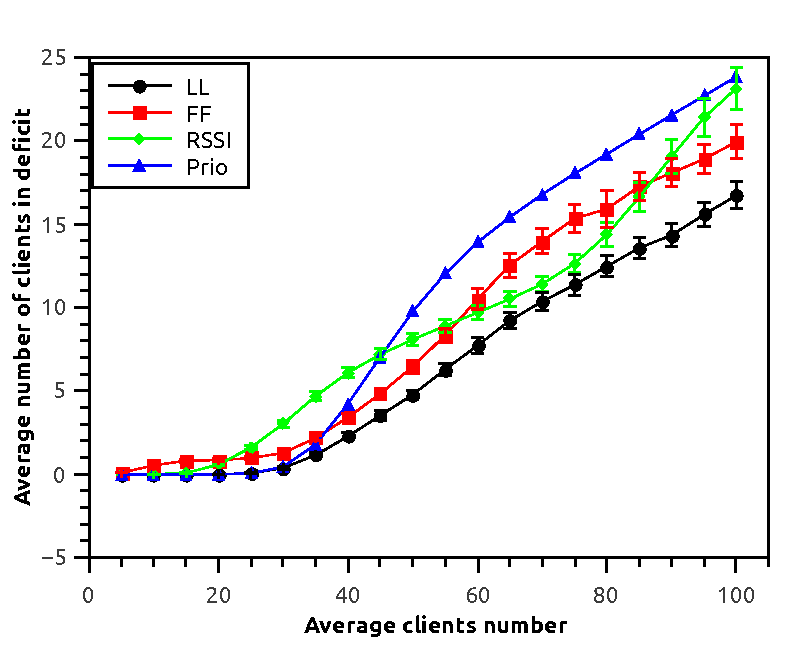
\includegraphics[scale=0.24]{Figures/online/fix/v1/nb_deficit/Graphe-nb-deficit-c4}}
\caption{Results for online fix Nb clients in deficit}
\label{fig:results_online_fix_Nb_clients_deficit_v1} 
\end{figure*}

%===========================================================

%=====APs Max and std loads V1 ============
\begin{figure}[t!]
\centering \subfigure[Average Max APs loads]{\includegraphics[scale=0.31]{Figures/online/fix/v1/Graphe-max-load.pdf}}
\subfigure[Average STD APs loads]{\includegraphics[scale=0.31]{Figures/online/fix/v1/Graphe-std-load.pdf}}
\caption{Results for online fix APS MAX and STD loads}
\label{fig:results_online_fix_loads} 
\end{figure}

%===========================================================

%=========================================================
%==========online  random figures==================================

%=====througput   V1============
\begin{figure*}[t!]
\centering \subfigure[Average Aggregated throughput for all clients]{\includegraphics[scale=0.25]{Figures/online/random_dem_var/v1/throughput/Graphe-throughput.pdf}}
\hfil \subfigure[Average Aggregated throughput for classe 1 clients]{\includegraphics[scale=0.25]{Figures/online/random_dem_var/v1/throughput/Graphe-throughput-c1}}
\subfigure[Average Aggregated throughput for classe 2 clients]{\includegraphics[scale=0.25]{Figures/online/random_dem_var/v1/throughput/Graphe-throughput-c2}}
\hfil \subfigure[Average Aggregated throughput for classe 3 clients]{\includegraphics[scale=0.25]{Figures/online/random_dem_var/v1/throughput/Graphe-throughput-c3}}
\hfil \subfigure[Average Aggregated throughput for classe 4 clients]{\includegraphics[scale=0.25]{Figures/online/random_dem_var/v1/throughput/Graphe-throughput-c4}}
\caption{Results for online random throughput}
\label{fig:results_online_random_throughput_v1} 
\end{figure*}

%===========================================================

%=====deficit   V1============
\begin{figure*}[t!]
\centering \subfigure[Average Aggregated deficit for all clients]{\includegraphics[scale=0.24]{Figures/online/random_dem_var/v1/deficit/Graphe-deficit.pdf}}
\hfil \subfigure[Average Aggregated deficit for classe 1 clients]{\includegraphics[scale=0.24]{Figures/online/random_dem_var/v1/deficit/Graphe-deficit-c1}}
\subfigure[Average Aggregated deficit for classe 2 clients]{\includegraphics[scale=0.24]{Figures/online/random_dem_var/v1/deficit/Graphe-deficit-c2}}'
\hfil \subfigure[Average Aggregated deficit for classe 3 clients]{\includegraphics[scale=0.24]{Figures/online/random_dem_var/v1/deficit/Graphe-deficit-c3}}
\hfil \subfigure[Average Aggregated deficit for classe 4 clients]{\includegraphics[scale=0.24]{Figures/online/random_dem_var/v1/deficit/Graphe-deficit-c4}}
\caption{Results for online fix deficit}
\label{fig:results_online_random_deficit_v1} 
\end{figure*}

%===========================================================

%=====Nb Clients  deficit   V1============
\begin{figure*}[t!]
\centering \subfigure[Average Aggregated Nb clients in deficit for all clients]{\includegraphics[scale=0.24]{Figures/online/random_dem_var/v1/nb_deficit/Graphe-nb-deficit.pdf}}
\hfil \subfigure[Average Aggregated Nb clients in deficit for classe 1 clients]{\includegraphics[scale=0.24]{Figures/online/random_dem_var/v1/nb_deficit/Graphe-nb-deficit-c1}}
\subfigure[Average Aggregated Nb clients in deficit for classe 2 clients]{\includegraphics[scale=0.24]{Figures/online/random_dem_var/v1/nb_deficit/Graphe-nb-deficit-c2}}'
\hfil \subfigure[Average Aggregated Nb clients in deficit for classe 3 clients]{\includegraphics[scale=0.24]{Figures/online/random_dem_var/v1/nb_deficit/Graphe-nb-deficit-c3}}
\hfil \subfigure[Average Aggregated Nb clients in deficit for classe 4 clients]{\includegraphics[scale=0.24]{Figures/online/random_dem_var/v1/nb_deficit/Graphe-nb-deficit-c4}}
\caption{Results for online random Nb clients in deficit}
\label{fig:results_online_random_Nb_clients_deficit_v1} 
\end{figure*}

%===========================================================

%=====APs Max and std loads V1 ============
\begin{figure}[t!]
\centering \subfigure[Average Max APs loads]{\includegraphics[scale=0.31]{Figures/online/random_dem_var/v1/Graphe-max-load.pdf}}
\subfigure[Average STD APs loads]{\includegraphics[scale=0.31]{Figures/online/random_dem_var/v1/Graphe-std-load.pdf}}
\caption{Results for online random positions APs MAX and STD loads}
\label{fig:results_online_random_loads} 
\end{figure}

%===========================================================

\subsubsection{online scheme evaluation}
In this scenario, the clients arrive and depart during the lifetime of the application following Poisson arrivals law and exponential law for stay period in the system. The priorities and demands of the clients are also randomly chosen.

\paragraph{Fixed location scenario}
In this scenario evaluation, each arriving client is given link capacities with the 4 available Access Points as $\left\{130,52,26,6.5 \right\}$ respectively. The Figure\ref{fig:results_online_fix_throughput_v1}.a,b,c,d shown that similarly to the offline scenario, the three candidates schemes present better throughput performance compared to the RSSI scheme. In fact, the problem with the RSSI scheme is that all the clients are associated with the stronger signal Access Point while the other three schemes, namely our priority based one (Prio), Fittingness Factor based(FF) and least loaded (LL) try to balance the clients associations between all the Access Points. But on the other hand, the FF and LL schemes do not take priority into account while in the ours the higher priority clients are served at first. Recall here again that at the level of Access Points we apply max-min time fairness resource sharing with the three schemes and priority based max-min time fairness with our scheme. The Figure\ref{fig:results_online_fix_deficit_v1}.a,b,c,d,e confirm the same analysis, as the clients with high priority have less deficit in our scheme compared to the other schemes, and that RSSI based scheme has the higher value of deficit. The Figure\ref{fig:results_online_fix_Nb_clients_deficit_v1}.a,b,c,d,e depict that our scheme again promotes the high priority clients against less priority ones as the number of clients with deficit is less for the high priority ones, while the other schemes treat all the clients equally. But as said previously, the RSSI based presents the higher number of clients with deficit. Finally, Figure\ref{fig:results_online_fix_loads}.a,c confirm the well balancing of the three schemes Prio, FF, LL, compared to the RSSI scheme, as the maximum load Access Point value starts to be got at the density of 40 clients in the system, and at this level the standard deviation of the Access Points level become small which reflects the general overload of all the Access Points.  
 
\paragraph{Random location scenario}
In this scenario, each arriving client gets random capacities with the available Access Points. This randomness is at the favour of the RSSI based scheme to gets load balanced as the Figure\ref{fig:results_online_random_throughput_v1}.a,b,c,d,e depict, in addition to the deficit values of the Figure\ref{fig:results_online_random_deficit_v1}.a,b,c,d,e. On the other hand, our priority scheme presents less better performance for the aggregated values of throughput or deficit. As explained in the offline scheme, this is due to the promote of the clients with high priority levels at first and after getting their demand satisfied, the other less priority clients are given their demands. But this prioritisation could be at the price of monopolising the link resource for a higher period and don't leave resources for the other clients. In fact, a high priority client with a bad link capacity but with high capacity demand will get all the time resource of the Access point with which it is associated and the other clients will be associated without time to receive the downlink traffic. But this behaviour could be a must in some applications as motivated before. The Figure\ref{fig:results_online_random_Nb_clients_deficit_v1}.a,b,c,d,e depict the same previous analysis of the candidate schemes. Finally, the Figure\ref{fig:results_online_random_loads}.a,c shown that the candidates can perform the load balancing well when the clients are them selves uniformly distributed in the system. This remark applies specially for the RSSI scheme that has a bad behaviour for the fix location scenario seen previously.   

\section{Conclusion (me)}
\label{Conclusion}
The use of WLAN is knowing more and more reputation, specially with the offloading of operators traffic to decrease resources cost. On the other hand, the clients applications need more and more resources leading to denser networks formed by multi cells WLAN in which the clients should choose their Access Points.
In this study, the clients association to WLAN Access Points is tackled when taking clients QOS demands into account. Contrary to the standard IEEE in which the clients associate to the highest signal strength AP leading to performance degradation because of overload traffic, we propose to take optimal association decisions of clients centrally at the SDN controller according to the clients priorities and bandwidth demands in order to balance the Access Points load charges. We proposed an offline periodic strategy and another online real time one. Simulation comparisons of the schemes shows their superiority compared to the standard and some pertinent state of the art works, specially for the high priority clients that are supposed performing important activities. We plan in future to perform real experimental tests by integrating time fairness resource sharing at the Access Points (already performed) and the SDN controller association decisions, with also power control and channel selection optimisation. 

\bibliographystyle{IEEEtran}
\bibliography{contribution.bib}
\end{document}
